%%%%%%%%%%%%%%%%%%%%%%%%%%%%%%%%%%%%%%%%%%%%%%%%%%%%%%%%
%%% Cell Reports Methods manuscript (Cell Press LaTeX template v1.10)
%%% Reframed from a Cell Reports-style draft toward a reproducible methods article
%%%%%%%%%%%%%%%%%%%%%%%%%%%%%%%%%%%%%%%%%%%%%%%%%%%%%%%%

\documentclass[12pt,letterpaper]{article}
\usepackage[a4paper, total={7in, 10in}]{geometry}
\renewcommand{\familydefault}{\sfdefault}
\usepackage{graphicx}
\usepackage{helvet}
\usepackage{authblk}
\usepackage{hyperref}
\usepackage{amsmath}
\usepackage{amssymb}
\usepackage{amsthm}
\usepackage{booktabs}
\usepackage{orcidlink}
\usepackage[super,comma,sort&compress]{natbib}
\bibliographystyle{numbered}
\usepackage[right]{lineno}
\linenumbers

\newcommand{\splitname}[1]{\textit{#1}}
\newcommand{\modpath}[1]{\textit{#1}}
\newcommand{\includefigwide}[1]{%
  \includegraphics[width=0.85\linewidth,keepaspectratio]{#1}}

\newtheorem{theorem}{Theorem}
\newtheorem{proposition}[theorem]{Proposition}
\newtheorem{definition}[theorem]{Definition}

\makeatletter
\renewcommand{\maketitle}{\bgroup\setlength{\parindent}{0pt}
\begin{flushleft}
  \textbf{\@title}
  \@author
\end{flushleft}\egroup}
\makeatother

\title{GERM-BO: a reproducible border-aware adapter framework for genomic foundation models}
\date{}

\author[1,*]{Mingxuan Huang}
\author[2]{Jingchao Wang}
\author[3]{Yang Shi}
\affil[1]{Zhongshan School of Medicine, Sun Yat-sen University, Guangzhou, China}
\affil[2]{Department, Institution, City, Country}
\affil[3]{Department, Institution, City, Country}
\affil[*]{Lead contact and correspondence: }

\begin{document}
\maketitle

\section*{HIGHLIGHTS}
\begin{itemize}
\item GERM-BO adds border-aware compensation to LoRA adapters for genomic models
\item Overlap-based border scores identify directions vulnerable to outlier suppression
\item Controlled and strict splice benchmarks test utility beyond short k-mer shortcuts
\item Ablations and cross-backbone pilots define when label-free scoring is sufficient
\end{itemize}

\section*{SUMMARY}

We present GERM-BO, a reproducible adapter framework for fine-tuning genomic foundation models under limited compute. GERM-BO augments LoRA-style adaptation with a border-aware compensation channel that reallocates adapter capacity toward sequence directions likely to be weakened by activation outlier suppression. The framework includes three reusable components: overlap-based border scoring for DNA words, a practical sample-level compensation rule for existing genomic backbones, and benchmark protocols that separate genuine border-aware generalization from short k-mer shortcuts. Analytic combinatorics of overlapping DNA words provides the design principle: self-overlapping genomic tokens recur in local clusters, produce burst-like activation responses, and can lose task-relevant information after uniform suppression. Controlled border-aware experiments, strict splice-site evaluation, ablations, and cross-backbone pilots show that GERM-BO improves over LoRA when border structure is informative while also defining settings where label-free scoring remains insufficient.

\section*{eTOC BLURB}

Huang et al. introduce GERM-BO, a reproducible border-aware adapter framework for genomic foundation models. GERM-BO uses DNA word overlap to guide LoRA-compatible compensation, improving adaptation when border-rich sequence structure is informative and exposing limits of label-free score estimation.

\section*{KEYWORDS}

genomic foundation model, computational method, resource efficient adaptation, DNA word overlap, outlier suppression, low rank compensation

\section*{INTRODUCTION}

Genomic foundation models have made pretrained sequence representations useful for regulatory elements, promoters, splice sites, and chromatin related prediction problems~\cite{dnabert2021,dnabert22023,nucleotidetransformer2024,hyenadna2024,jaganathan2019spliceai}. Their practical use, however, often depends on parameter-efficient adaptation rather than full fine-tuning. Recent resource-efficient models show that adaptation and quantization can be made cheaper when activation outliers are suppressed during pretraining and fine tuning~\cite{germ2025,dettmers2022llm,int8outlier2022,lian2024medpeft}. This strategy is attractive for computational genomics because many users have a single workstation, a small adapter budget, and limited labeled data.

The missing methodological ingredient is sequence structure awareness. Genomic tokens are not generic words~\cite{lindsey2025impact}. They arise from a finite alphabet, often correspond to motifs or merged subwords, and can have strong self-overlap, a property studied in the combinatorics of words and pattern matching~\cite{guibas1981string,Dai2011}. A token with strong border structure can recur after a short shift, producing clustered local occurrences related to motif clustering and regulatory grammar~\cite{encode2012integrated,zhou2015predicting}. When a model assigns large aligned responses to these clustered occurrences, activations are not isolated extremes but burst-like events~\cite{bondarenko2021understanding,aldous1989poisson,dettmers2022llm}. A large response can therefore be both a computational outlier and a task-relevant genomic signal~\cite{Kinney2010}.

This observation exposes a method gap in outlier-free genomic adaptation. Existing work shows that suppressing activation outliers improves average low-rank adaptation and quantization efficiency~\cite{germ2025,lora2022}. It does not specify which genomic directions are most affected by this suppression, how those directions can be estimated from sequence information, or how an adapter should compensate them without increasing the trainable rank. A generic bound on norms or Lipschitz constants would not answer this question because such bounds are typically agnostic to discrete overlap structure in sequences~\cite{bartlett2017spectrally} and do not include the overlap, threshold, and compensation variables that define this setting~\cite{allen2019learning,golowich2018size}.
As illustrated in Fig.~\ref{fig:motivation}, self-overlapping tokens induce clustered occurrences that give rise to burst-like activations, which are disproportionately suppressed by uniform clipping, leading to substantial loss of task-relevant signals in border-rich directions.

\begin{figure}[htbp]
\centering
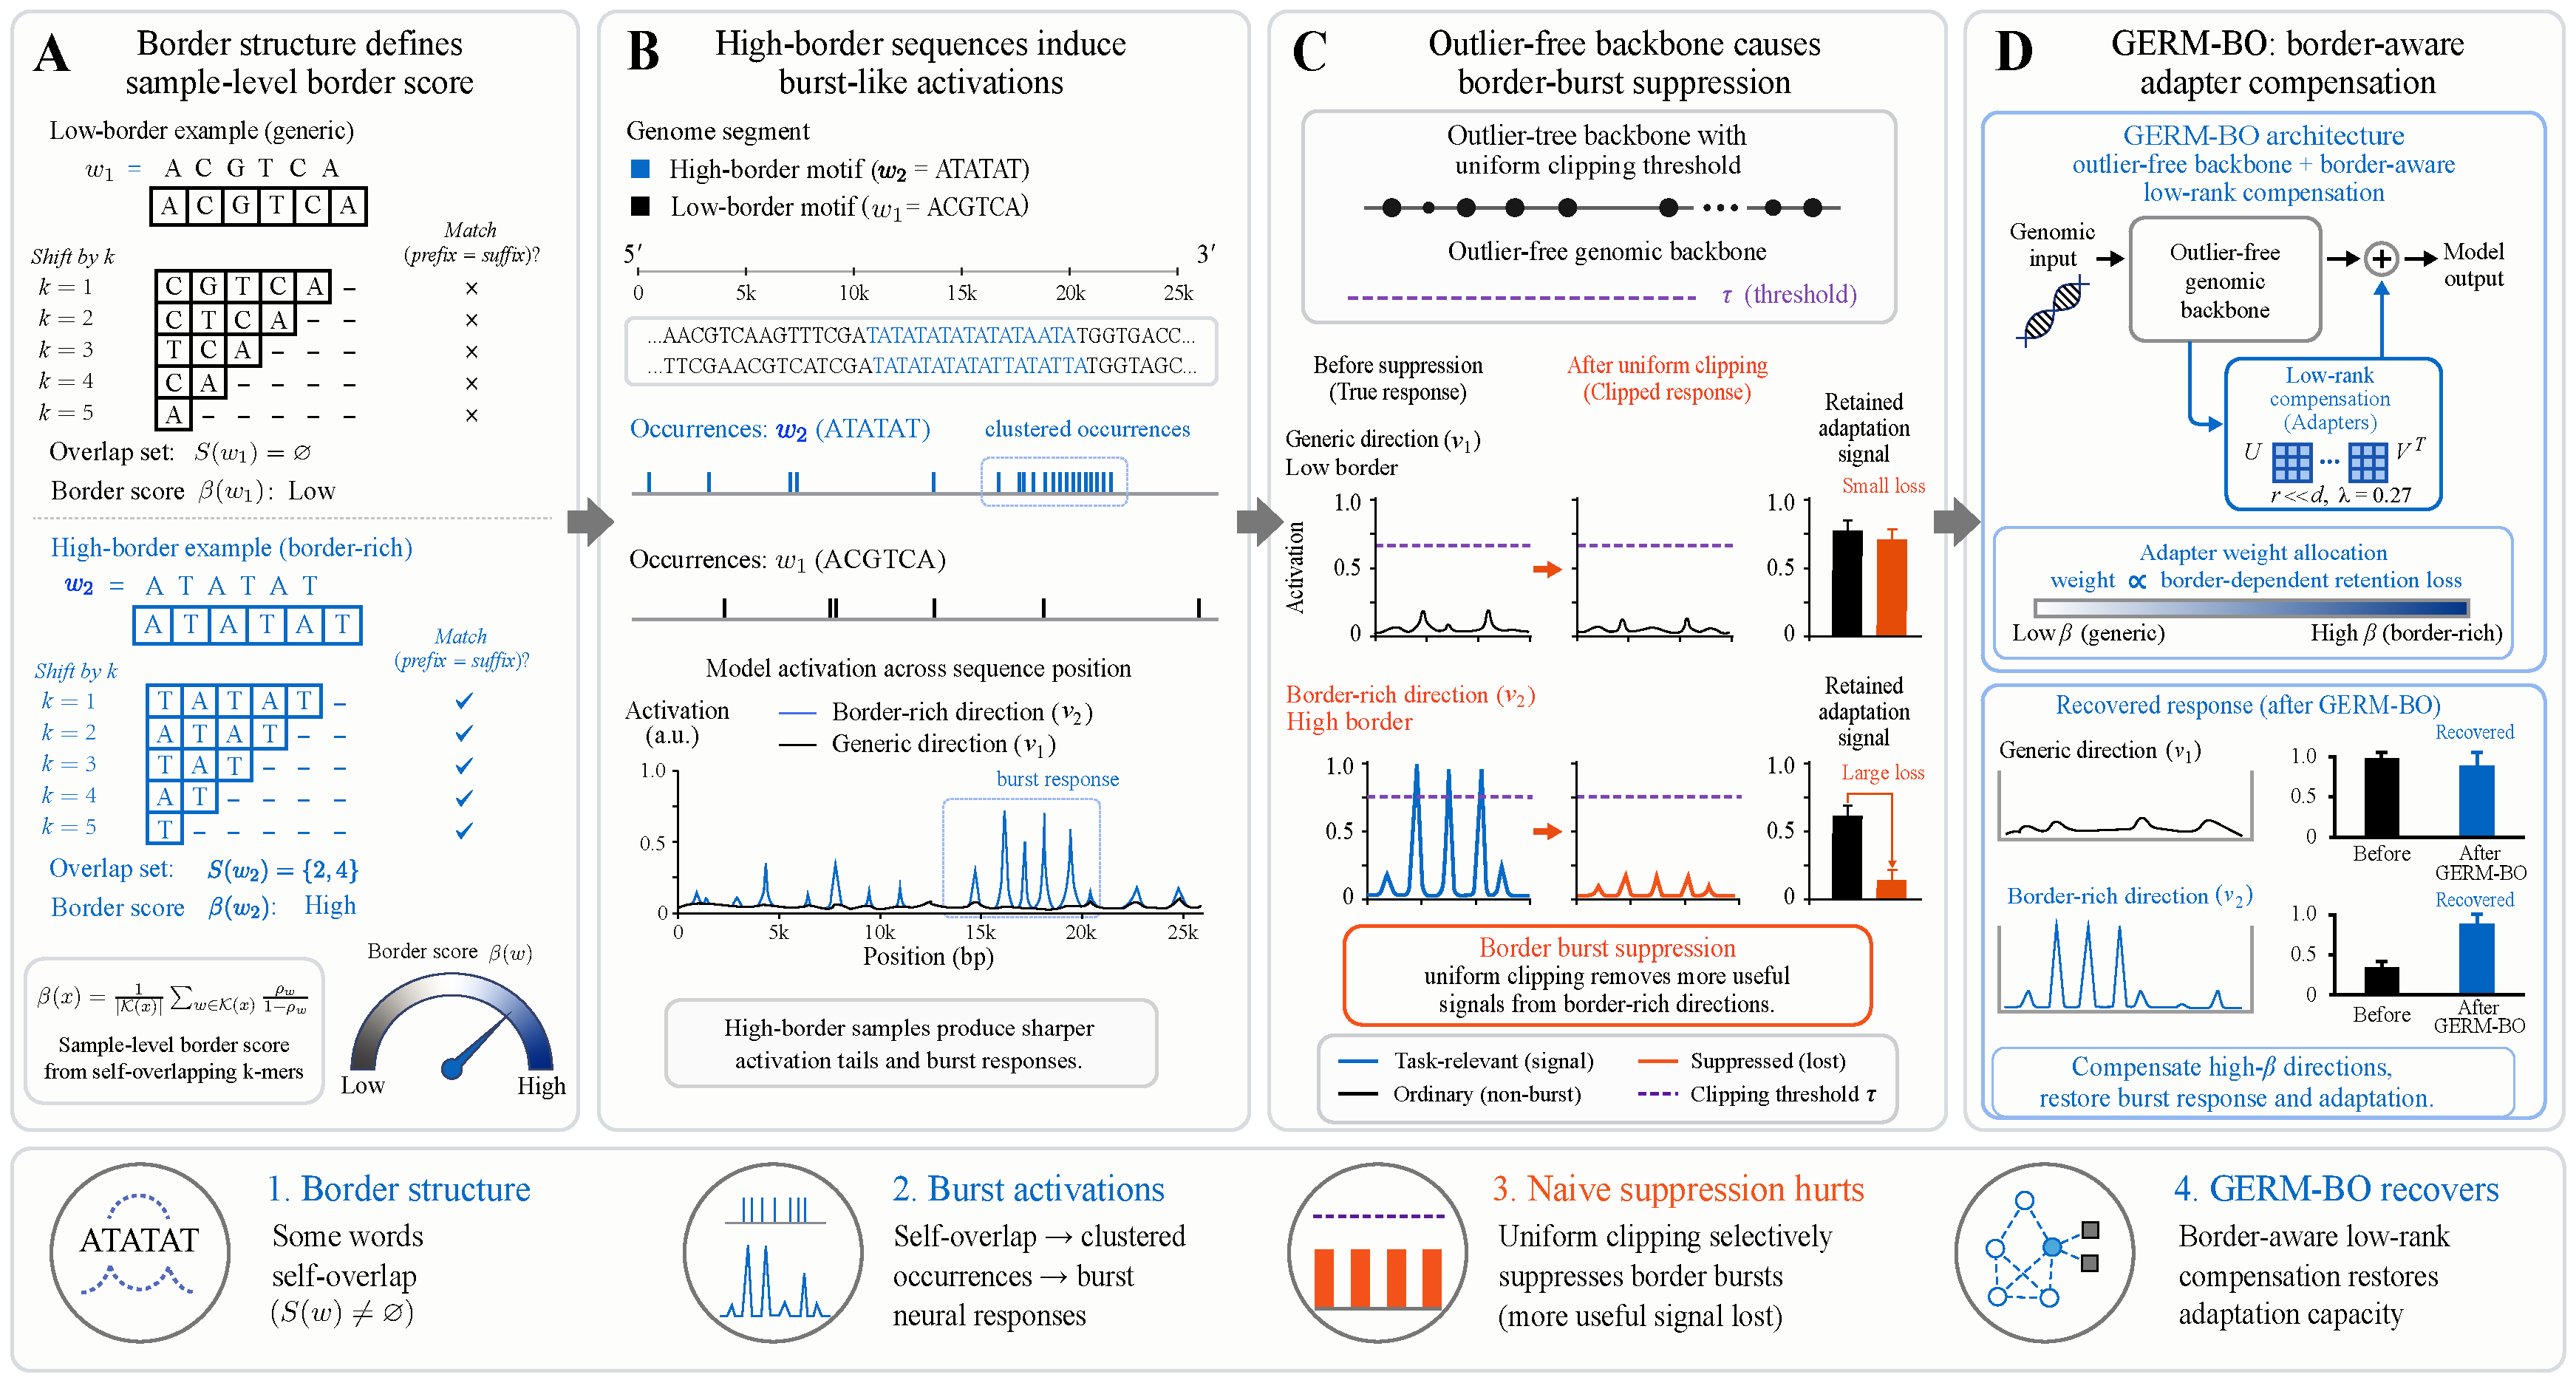
\includegraphics[width=0.85\linewidth]{fig1.pdf}
\caption{Border-induced burst activations caused by self-overlapping genomic tokens and the limitation of uniform outlier suppression. High-border sequences (e.g., repetitive motifs such as ATATAT) induce clustered occurrences and burst-like neural activations. Uniform clipping suppresses these bursts but disproportionately removes task-relevant signals in border-rich directions. GERM-BO addresses this issue via border-aware low-rank compensation that selectively restores suppressed informative components.}
\label{fig:motivation}
\end{figure}



Here we introduce GERM-BO as a reusable adapter framework for this problem. The framework keeps the outlier-free backbone and the LoRA rank budget unchanged, but adds a border-aware compensation factor to the adapter branch. Its design is guided by analytic combinatorics of overlapping DNA words: border geometry induces clustered occurrence laws, these laws inflate response variance in a token-specific way, and outlier suppression can reduce retained adaptation information on high-border genomic directions. We call this failure mode border-burst suppression and use it to derive the compensation rule.

The goal of GERM-BO is methodological rather than solely explanatory. It provides a score channel, an implementation path, and an evaluation protocol that can be reused with existing genomic backbones. The theory links the overlap set of a genomic word, the suppression threshold, and adapter compensation weights; the experiments test when this link translates into measurable gains and when label-free score estimation remains too weak.

Our contributions are summarized as follows.
\begin{itemize}
\item We provide a reusable border-scoring framework for genomic tokens and show how overlap structure determines short-range recurrence and burst statistics.
\item We derive border-burst suppression as the design principle for compensation and prove that retained adaptation information decreases with border score under a broad class of outlier-suppression maps.
\item We implement GERM-BO as a LoRA-compatible compensation channel that can use metadata, activation-derived, or label-free sequence-estimated scores without changing the backbone.
\item We validate the method with controlled border-aware tasks, a strict 3-mer-balanced splice benchmark, ablations, resource measurements, and cross-backbone pilots that define both utility and scope.
\end{itemize}

Recent genomic foundation models extend transformer style pretraining to large collections of DNA sequences and downstream tasks across species and assays~\cite{dnabert2021,dnabert22023,nucleotidetransformer2024,hyenadna2024,genomicsurvey2025}. They differ in tokenizer design, context handling, and architectural efficiency, but they share the goal of transferring sequence level priors to small labeled tasks. For instance, DNABERT~\cite{dnabert2021} pioneered the use of BERT-style masked language modeling on DNA, employing fixed-length k-mer tokenization. Its successor, DNABERT-2~\cite{dnabert22023}, introduced a more efficient Byte Pair Encoding (BPE) tokenizer and a novel positional encoding scheme to better capture genomic semantics. Other models expand context length or evaluation scope through alternative sequence operators and broader benchmarks~\cite{hyenadna2024,genomicsurvey2025}. HyenaDNA~\cite{hyenadna2024}, for example, replaces attention with long convolutional filters, enabling it to process sequences up to 1 million tokens, far beyond the typical transformer context window. Parallel work in medical imaging has pursued multimodal fusion of imaging and molecular or genomic signals for diagnosis and prognosis~\cite{wei2023tmi,chen2022pathomic,imaginggenetics2022,hmf2022}, showing that sequence level priors and imaging phenotypes are increasingly studied within a unified predictive framework. These studies mainly evaluate predictive accuracy and efficiency at the model level.

Our work differs from this line because we study a token level mechanism that is specific to genomic overlap structure. The object of analysis is not only the backbone architecture but also the combinatorial geometry of genomic words that produce clustered activations.

Parameter efficient adaptation and low bit quantization are important tools for deploying large pretrained models under limited resources~\cite{adapters2021,lora2022,qlora2023,lian2024medpeft}. Adapter layers~\cite{adapters2021} insert small, trainable modules between transformer layers, while LoRA~\cite{lora2022} approximates weight updates via low-rank decomposition ($\Delta W = B A$ with $B \in \mathbb{R}^{d_{\mathrm{out}}\times r}$ and $A \in \mathbb{R}^{r\times d_{\mathrm{in}}}$), drastically reducing the number of trainable parameters. QLoRA~\cite{qlora2023} further combines quantization with LoRA for memory-efficient fine-tuning of extremely large models. Recent variants reweight or gate adapter directions at the token or task level~\cite{stickland2019bert,ilharco2022editing,he2022unified}, but they are not designed around genomic overlap geometry. In the genomic setting, GERM shows that removing activation outliers during pretraining and fine tuning can improve both low rank adaptation and quantization robustness~\cite{germ2025}. In medical imaging, similar transfer learning studies report that low rank adaptation can match or exceed full fine tuning while updating only a small fraction of parameters~\cite{lian2024medpeft,yang2023hypernet,liu2025imitate}. This is achieved through techniques like activation clipping and normalization, which smooth the optimization landscape. This is a strong practical direction because it directly targets resource constrained fine tuning rather than only improving accuracy at unlimited scale.

Our work differs from this line because we ask which genomic directions are suppressed by the same mechanism that improves average efficiency. The answer depends on border induced burst structure, which is not captured by standard PEFT analyses that treat tokens as generic independent features.

Genomic sequences contain abundant repetitive and self-similar structure, from transposable elements and tandem repeats to clustered regulatory motifs~\cite{encode2012integrated,jurka2005repbase,smit1996repeatmasker}. Such structure can inflate local recurrence of overlapping words and create burst-like occurrence patterns that are biologically meaningful rather than random noise~\cite{zhou2015predicting,Kinney2010}. Methods for repeat masking and motif clustering are widely used in genome annotation, but they are rarely connected to parameter efficient adaptation of foundation models. Our overlap-based view is complementary: it explains how repeat-prone token geometry can interact with outlier suppression during adaptation, and why compensation should be border-aware rather than uniform.

Analytic combinatorics of word overlap studies how borders, autocorrelation, and recurrence determine the statistics of repeated patterns in finite alphabet sequences~\cite{guibas1981,wordstats2022}. The foundational work by Guibas and Odlyzko~\cite{guibas1981} provides generating functions to count strings with specified autocorrelation (border) properties. Modern extensions, such as those surveyed in~\cite{wordstats2022}, apply these methods to compute exact and asymptotic distributions of pattern occurrences in random texts. These tools have been used to study waiting times, cluster counts, and rare event probabilities for strings with internal overlap. They are well suited to DNA because the alphabet is small and the same motif can reappear after a short shift if its prefix matches its suffix.

Our work differs from this line because we do not stop at pattern counting. We connect overlap combinatorics to activation tails, outlier suppression, and low rank compensation in genomic foundation models. This closes a model specific chain from genomic token statistics to resource efficient adaptation.

\section*{RESULTS}

The Results are organized around method use and validation. We first define the border-burst mechanism that determines when compensation is needed, then specify the GERM-BO adaptation rule, implementation path, and reproducibility package. We then validate the method in controlled border-aware settings, test label-free scoring on real genomic benchmarks, and close with sensitivity, resource, and cross-backbone analyses that define the practical scope of the framework.

\subsection*{Border-burst suppression defines the target for compensation}

GERM-BO starts from a token-level observation: a genomic word with strong self-overlap can recur after a short shift, producing clustered local occurrences rather than isolated hits. For a word $w=w_1\cdots w_m$, we define its overlap set as
\begin{equation}
S(w) = \{\ell \in \{1,\ldots,m-1\} \mid w_{1:m-\ell} = w_{\ell+1:m}\}.
\label{eq:overlapset}
\end{equation}
Under a stationary Markov background, each valid overlap shift has a short-range continuation probability $q_w(\ell)=\mathbb{P}(I_{t+\ell}(w)=1\mid I_t(w)=1)$. We summarize the total continuation mass and border score as
\begin{equation}
\rho_w = \sum_{\ell \in S(w)} q_w(\ell),
\qquad
\beta_w = \frac{\rho_w}{1-\rho_w},
\label{eq:beta}
\end{equation}
where $\rho_w<1$. In the rare-word renewal approximation, the expected local cluster length is $1/(1-\rho_w)=1+\beta_w$ (Document S1). Thus $\beta_w$ is the scalar quantity that GERM-BO uses to identify directions whose signal is likely to arrive in bursts rather than as independent token events.

Outlier suppression can attenuate these bursty directions. Let $q_{\tau}$ be a clipping or smooth-suppression map with derivative $\phi_{\tau}$, let $a_w$ be the activation response aligned with word $w$, and let $g_w$ be the corresponding task-loss gradient. We measure the retained task information after suppression by
\begin{align}
I_w(\tau) &= \mathbb{E}_{(X,Y)\sim \mathcal{D}}\!\left[\phi_{\tau}(a_w(X))^2 g_w(X,Y)^2\right], \label{eq:fisherretained}\\
R_w(\tau) &= \frac{I_w(\tau)}{I_w(\infty)}. \label{eq:retention}
\end{align}
The core theoretical result is that, under a scale model $a_w\overset{d}{=}b_0(1+\beta_w)Z$ and the independence assumptions stated in Document S1, $R_w(\tau)$ is nonincreasing in $\beta_w$ for fixed $\tau$.
\begin{theorem}\label{thm:fisher}
Under the scale and independence assumptions above, high-border directions retain no more post-suppression Fisher information than low-border directions: if $\beta_{w_1}\leq\beta_{w_2}$, then $R_{w_1}(\tau)\geq R_{w_2}(\tau)$ for every fixed suppression threshold $\tau>0$.
\end{theorem}
This motivates border-burst suppression: the same outlier-control mechanism that improves average efficiency can disproportionately reduce information in high-border genomic directions. Full variance calculations, response-channel bounds, and proofs are provided in Document S1; the main text keeps only the quantities needed to specify and evaluate the method.

\begin{figure}[htbp]
\centering
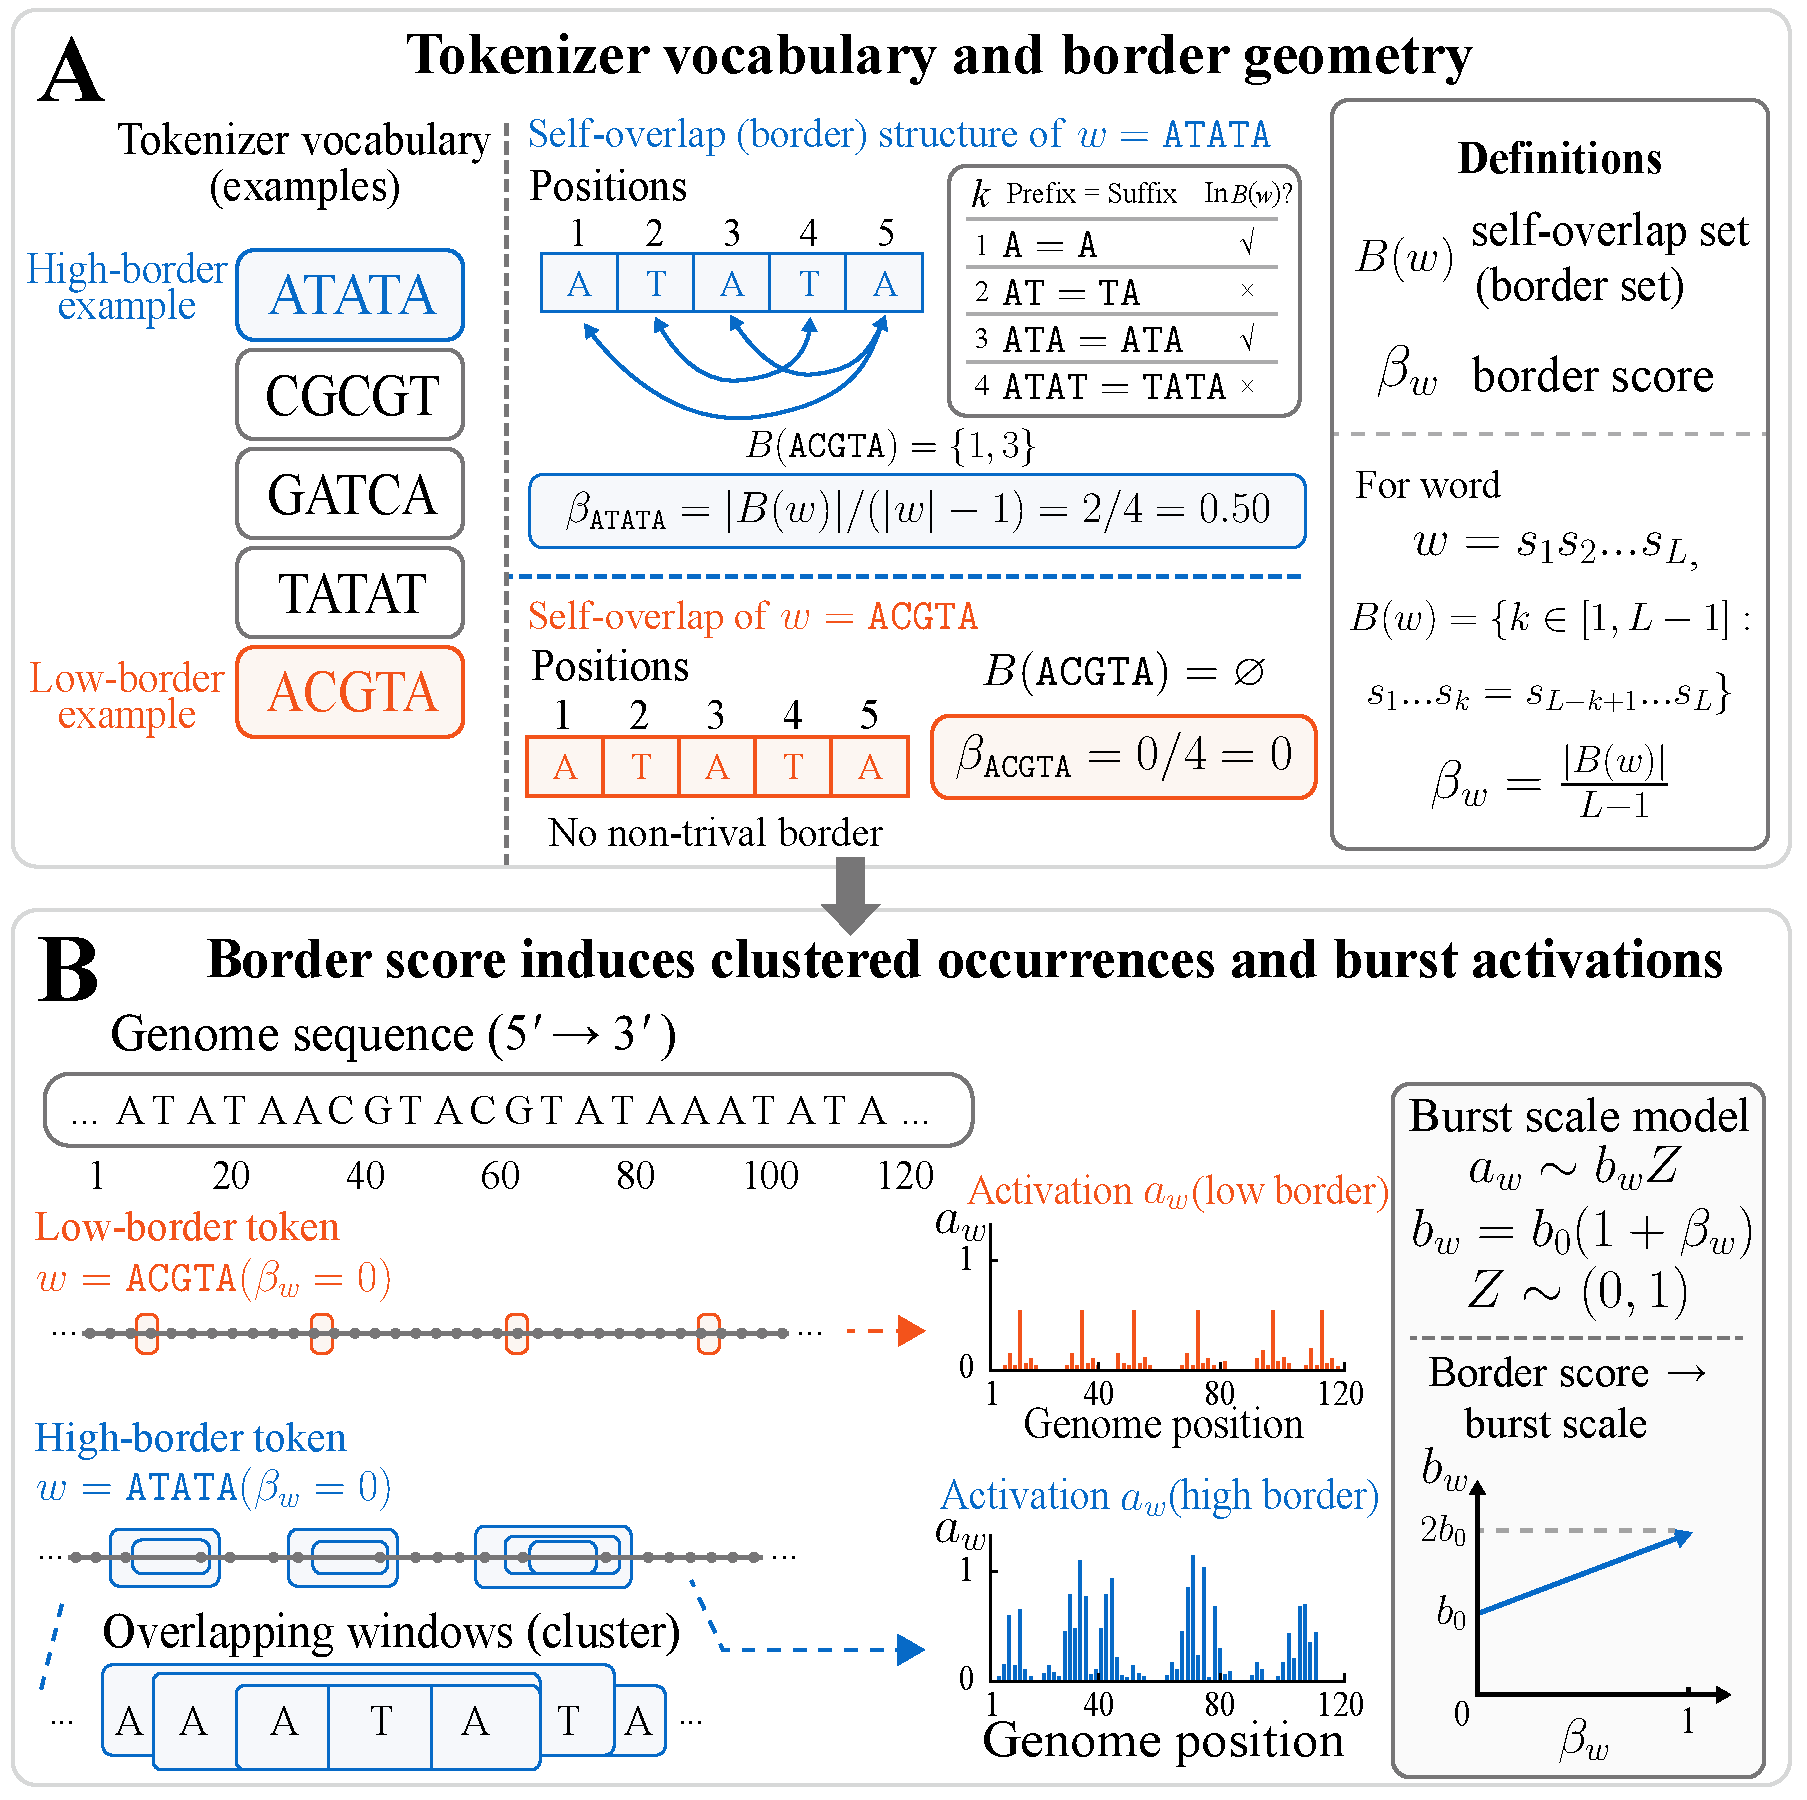
\includegraphics[width=0.85\linewidth]{fig2_ab.pdf}
\caption{Token-level border structure and burst modeling in GERM-BO. \textbf{(A)}, Illustration of genomic token overlap and the definition of the border score $\beta_w$. High-border tokens (e.g., repetitive motifs) induce clustered occurrences in sequence space. \textbf{(B)}, Modeling of border-induced activation bursts and their suppression. The retention of task-relevant information, $R_w(\tau)$, decreases monotonically with the border score $\beta_w$ under uniform outlier clipping, revealing the \emph{border-burst suppression} failure mode.}
\label{fig:method_border_modeling}
\end{figure}

\subsection*{GERM-BO workflow and adaptation rule}

GERM-BO modifies a LoRA-style adapter by reweighting the adapter branch with a border-derived compensation signal. For a linear map $W$, standard LoRA uses
\begin{equation}
\Delta W = B A,
\label{eq:lora}
\end{equation}
where $B$ and $A$ are low-rank factors. The idealized token-aligned form of GERM-BO is
\begin{equation}
\Delta W = B A \Gamma,
\label{eq:GERM-BO}
\end{equation}
where $\Gamma$ is diagonal in a token-aligned basis and assigns larger weights to directions with stronger predicted retention loss. This keeps the trainable rank budget unchanged while changing how adapter capacity is allocated across genomic directions.

Document S1 derives an optimal compensation rule from a local retained-information surrogate. The practical consequence is simple: because Theorem~\ref{thm:fisher} makes $R_w(\tau)$ nonincreasing in $\beta_w$, higher-border directions should receive larger compensation. When $R_w(\tau)$ is not calibrated for each token, we use the monotone approximation
\begin{equation}
\gamma_w = (1+\beta_w)^{\alpha},
\label{eq:powerlaw}
\end{equation}
with a single exponent $\alpha>0$ (Fig.~\ref{fig:method_compensation}).

\begin{figure}[htbp]
\centering
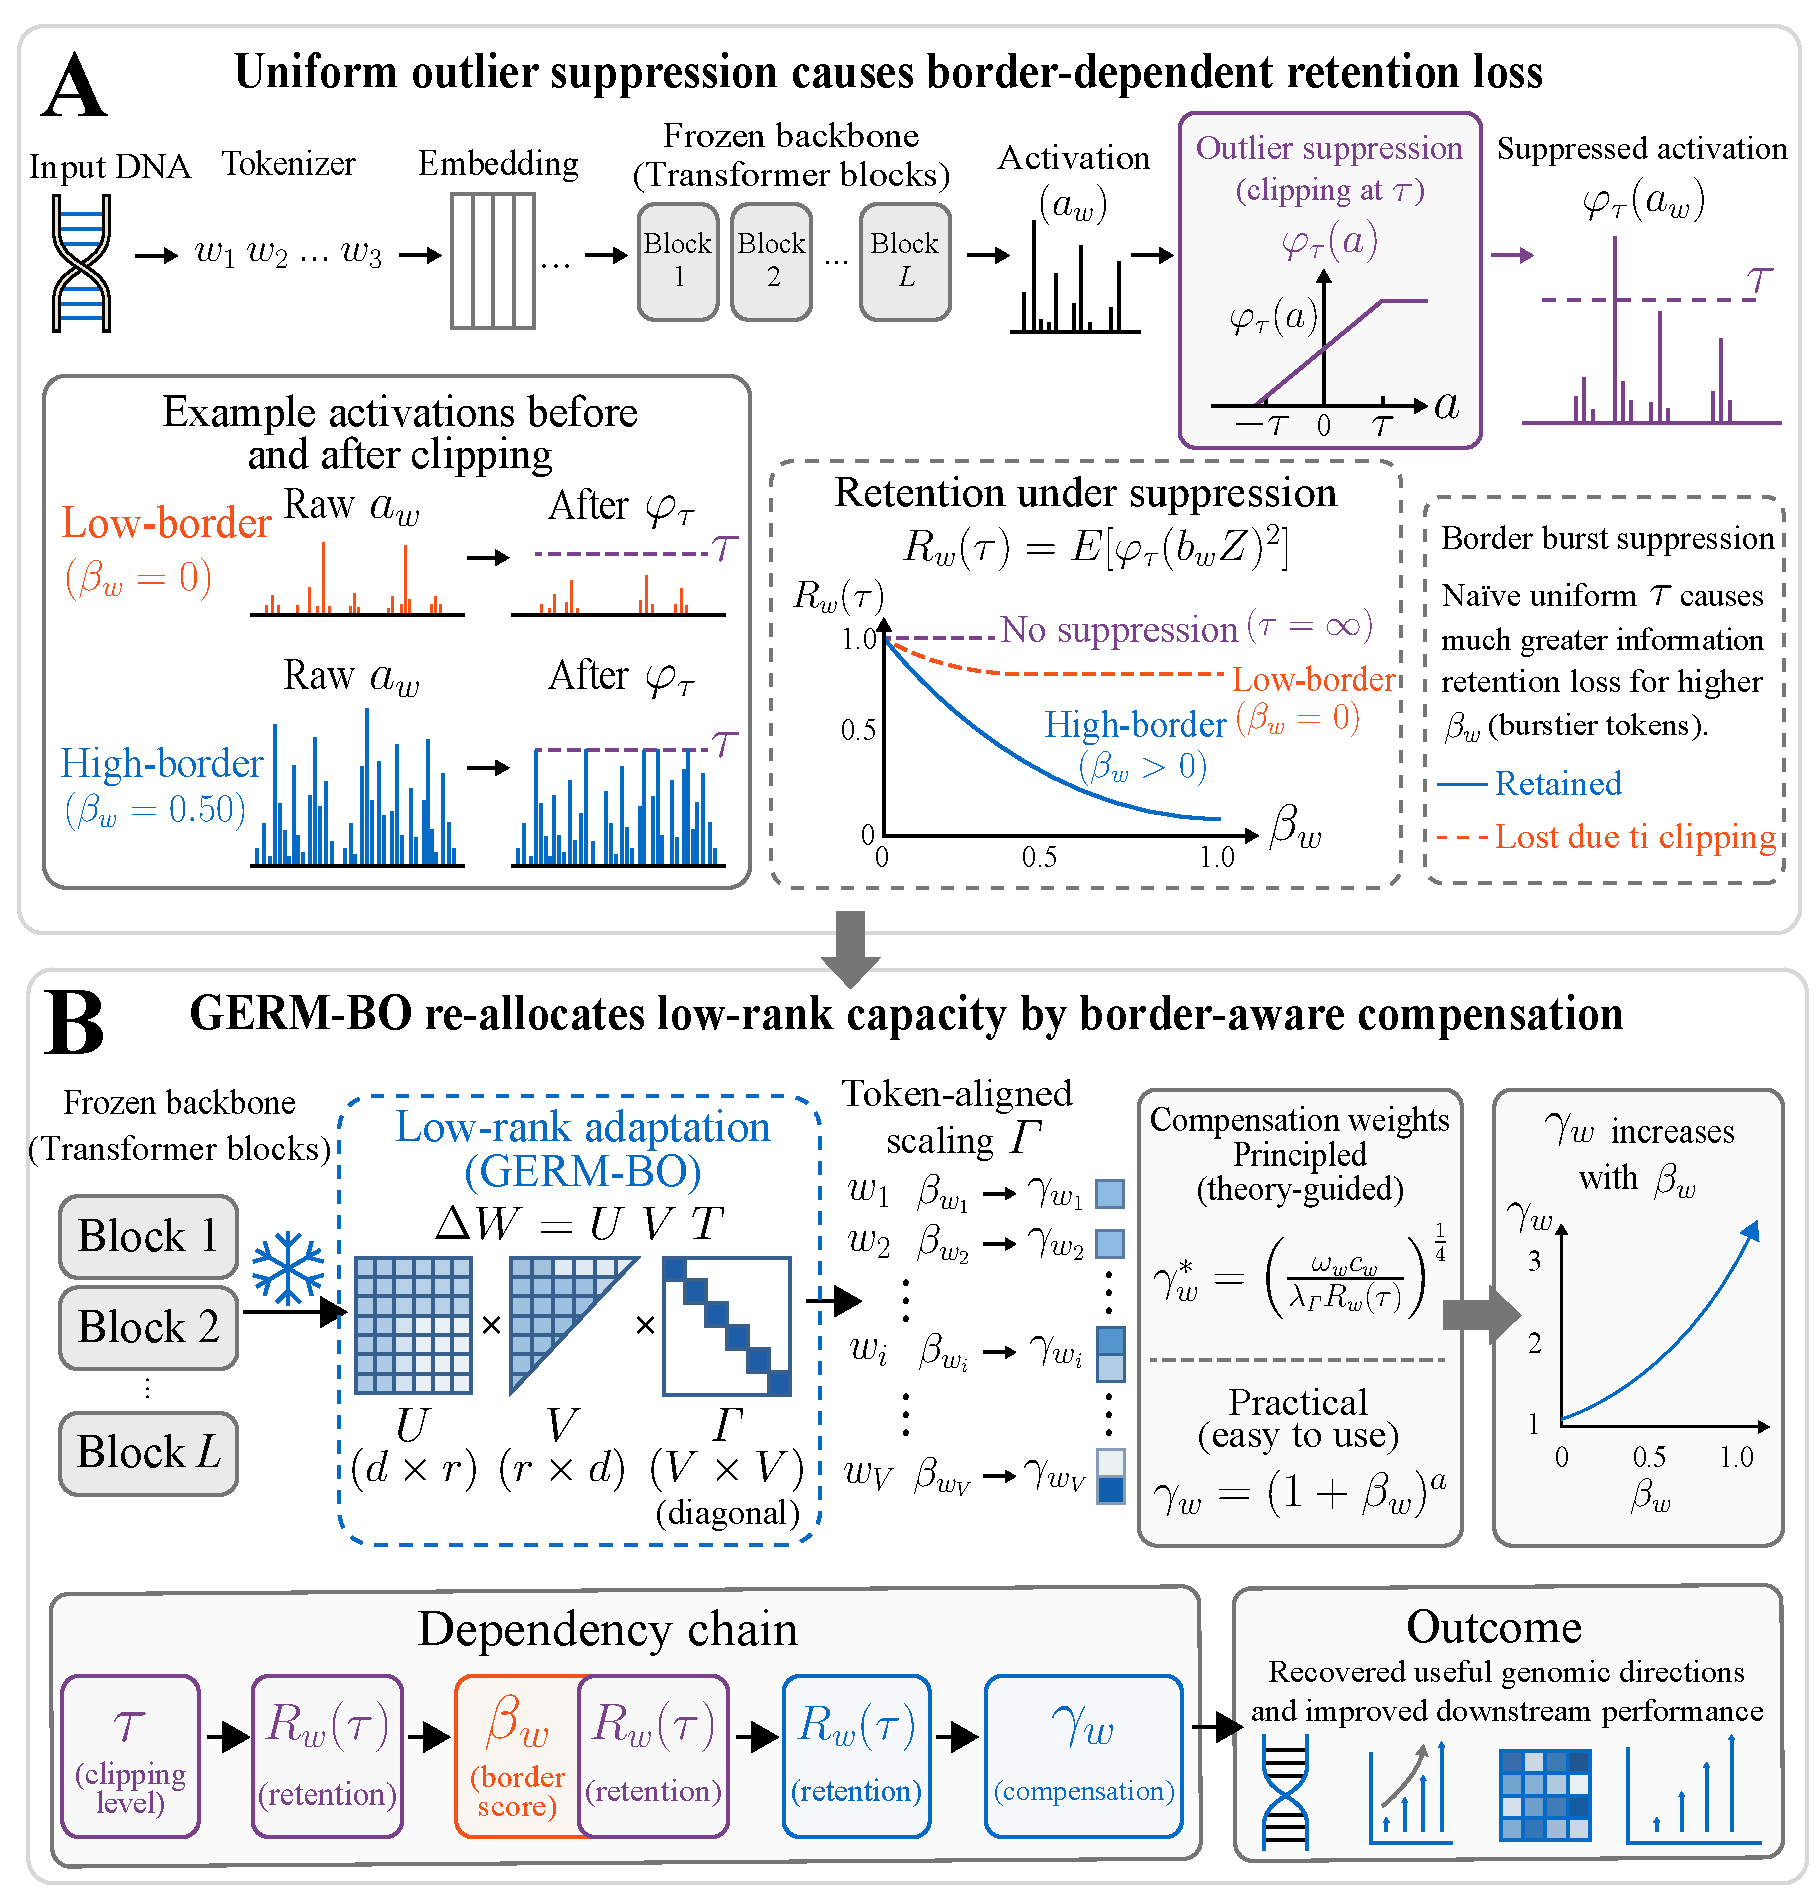
\includegraphics[width=0.85\linewidth]{fig2_cd.pdf}
\caption{Border-aware low-rank compensation in GERM-BO. \textbf{(C)}, Framework of the compensation module. The standard low-rank update $\Delta W = BA$ is augmented with a diagonal compensation matrix $\Gamma$, yielding $\Delta W = BA\Gamma$ in the theoretical token-aligned basis. The entries $\gamma_w$ of $\Gamma$ are computed based on the border score $\beta_w$ and the retained information $R_w(\tau)$. \textbf{(D)}, Adaptive allocation of adaptation capacity. Compensation weights $\gamma_w$ increase with $\beta_w$, strategically reallocating the low-rank budget to restore suppressed signals in high-border, information-rich directions.}
\label{fig:method_compensation}
\end{figure}

\subsubsection*{Theory-to-implementation mapping.}
The deployed trainer does not instantiate a full vocabulary-aligned $\Gamma$ matrix. Instead, it applies the same low-rank factors $B$ and $A$ as LoRA and multiplies the intermediate LoRA branch by a per-sample compensation factor
\begin{equation}
c(x) = \mathrm{clip}\!\left(1 + \lambda_{\mathrm{comp}}\left(\frac{s(x)}{\mathbb{E}_{\mathrm{batch}}[s]}-1\right),\, c_{\min},\, c_{\max}\right),
\label{eq:implcomp}
\end{equation}
where $s(x)$ is a metadata, activation-derived, or sequence-estimated border score. The forward update is $y = W x + \mathrm{scale}\cdot B(A(\mathrm{dropout}(x))\cdot c(x))$, with $c(x)$ broadcast to valid tokens in the sequence. Thus the operational method is a scalar score channel on the LoRA branch rather than a full diagonal embedding-coordinate matrix. The theoretical budget parameter is not identical to the implemented compensation strength $\lambda_{\mathrm{comp}}$. We use $\lambda_{\mathrm{comp}}=0.27$ with $c_{\min}=0.73$ and $c_{\max}=1.42$ in the main controlled runs, and quantile-normalized scores clipped to $[0.8,1.2]$ on the strict splice split. Tokenizer alignment, Markov-background score estimation, and proof details are provided in Document S1.

\subsubsection*{Reproducibility package and intended use.}
GERM-BO is intended to be used as a drop-in adapter path for existing genomic foundation model fine-tuning scripts. The submission package will include the trainer, adapter implementation, border-score utilities, processed split builders, run configurations, and scripts for regenerating the main result tables and figures. Each reported experiment is tied to a YAML configuration and a single-GPU command. The debug workflow first runs on mock data, then on the controlled border-aware splits, and finally on the strict external splice split. This staged design is meant to let users verify installation, reproduce the core mechanism, and then evaluate whether a new genomic task contains enough border-associated signal to benefit from compensation.

\subsection*{Evaluation design and controlled validation}

We evaluate GERM-BO in two regimes. The first is a \emph{controlled border-aware setting}, where a sample-level border score is available from task construction and can be used to test the mechanism under ideal conditions. The second is a \emph{real external benchmark setting}, where the score must be estimated from sequence information.

All experiments use a pretrained genomic backbone based on DNABERT-2~\cite{dnabert22023}. We compare against standard LoRA-style baselines and GERM-style outlier-suppression baselines. All runs use a single GPU with \texttt{CUDA\_VISIBLE\_DEVICES=3}. We additionally replicate the oracle-metadata \splitname{border\_hard} protocol on Nucleotide Transformer v2 50M and HyenaDNA tiny backbones (Section~Results, cross-backbone replication). For binary controlled tasks we report test accuracy and F1; for the 3-class splice benchmark we report test accuracy and macro-F1. Unless otherwise stated, results are reported as mean $\pm$ standard deviation over multiple seeds. For key pairwise comparisons, we additionally report paired bootstrap confidence intervals and win rates.

Default adapter hyperparameters are LoRA rank $r=8$, scaling $\alpha=16$, dropout $0.05$, and compensation strength $\lambda_{\mathrm{comp}}=0.27$ with clip range $[c_{\min},c_{\max}]=[0.73,1.42]$ on controlled metadata runs. On the strict splice split we use train-quantile normalization with clip $[0.8,1.2]$. The theoretical suppression threshold $\tau$ is not tuned inside the trainer; we estimate it post hoc from activation snapshots (Results). The power-law exponent $\alpha$ in Equation~\eqref{eq:powerlaw} is likewise not tuned during training; $\lambda_{\mathrm{comp}}$ is the operational compensation knob corresponding to Equation~\eqref{eq:implcomp}.

The controlled suite contains \splitname{border\_easy}, \splitname{border\_medium}, \splitname{border\_hard}, and an enlarged \splitname{hard\_border\_large} split used for the final main result. The external study focuses on \splitname{splice\_sites\_all}. Since the original splice split is strongly affected by short-range $3$-mer shortcuts, our final external evaluation uses a stricter \splitname{3-mer-balanced} split, following recent deep learning splice benchmarks~\cite{jaganathan2019spliceai,zhang2023pangolin}.

\subsubsection*{Controlled border-aware benchmarks}

Table~\ref{tab:controlled-main} reports the main result on \splitname{hard\_border\_large}. The corresponding visual comparison and performance trends are shown in Fig.~\ref{fig:controlled_main_mechanism}A and Fig.~\ref{fig:controlled_main_mechanism}C, where metadata-driven GERM-BO consistently achieves the strongest performance across metrics and difficulty regimes. We compare the three main methods: LoRA (baseline), GERM-BO (Act) (activation-derived), and GERM-BO (Meta) (metadata-driven). The final setting uses metadata border scores, compensation strength $\lambda_{\mathrm{comp}}=0.27$, and \modpath{attention.output + classifier} as the target module set.

\begin{table}[htbp]
\centering
\caption{Controlled main result on the enlarged \splitname{hard\_border\_large} split. Results are reported over 13 seeds.}
\label{tab:controlled-main}
\small
\begin{tabular}{lccc}
\toprule
Method & Seeds & Accuracy & F1 \\
\midrule
Baseline LoRA & 13 & $0.8377 \pm 0.0544$ & $0.8300 \pm 0.0725$ \\
Activation-derived GERM-BO & 13 & $0.8918 \pm 0.0255$ & $0.8896 \pm 0.0276$ \\
Metadata-driven GERM-BO & 13 & $\mathbf{0.9519 \pm 0.0443}$ & $\mathbf{0.9493 \pm 0.0483}$ \\
\bottomrule
\end{tabular}
\end{table}





The gain is substantial and stable. Relative to Baseline LoRA, metadata-driven GERM-BO improves accuracy by $+0.1142$ with bootstrap $95\%$ confidence interval $[+0.0703, +0.1593]$ and wins on $92.3\%$ of seeds. Relative to the activation-derived variant, the gain is still clear: $+0.0601$ accuracy with bootstrap $95\%$ confidence interval $[+0.0361, +0.0835]$. This establishes the main controlled claim: when a meaningful border score is available, border-aware compensation produces a strong improvement. The mechanism-level comparison in Fig.~\ref{fig:controlled_main_mechanism}B further shows that the gain is specific to correctly aligned border-aware compensation rather than a generic architectural effect.

\begin{figure}[htbp]
\centering
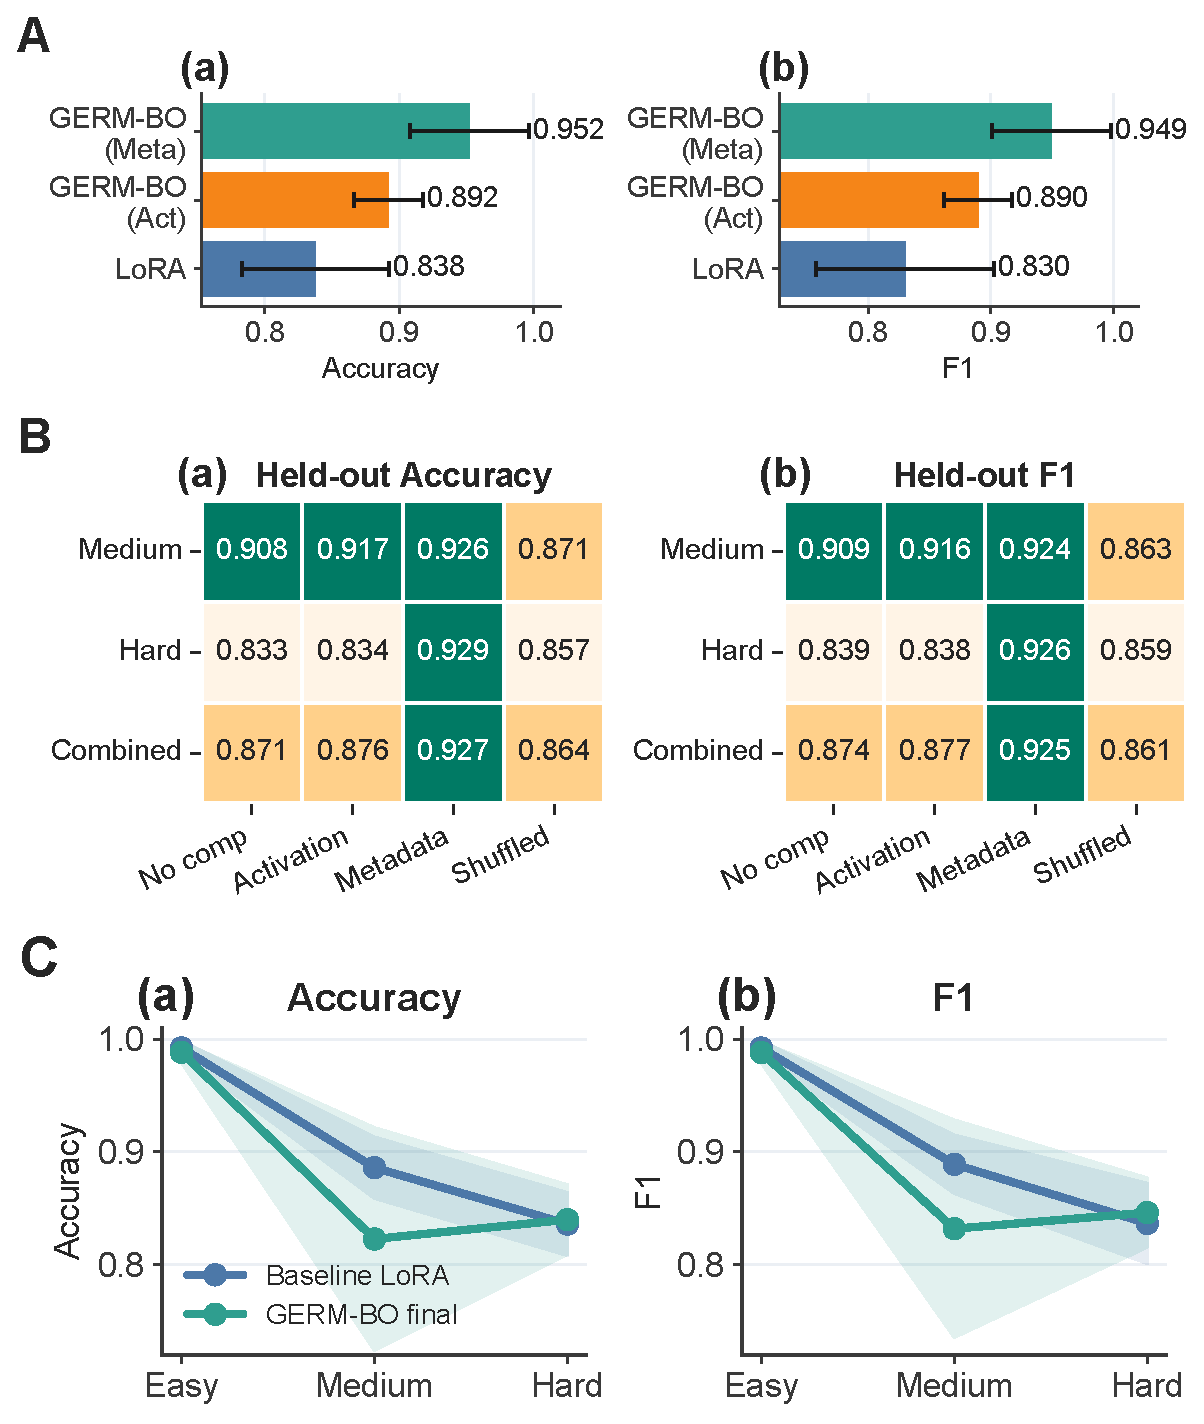
\includegraphics[width=0.85\linewidth]{010203.pdf}
\caption{Controlled border-aware main results and mechanism validation. \textbf{A}, controlled main results on \splitname{hard\_border\_large}, showing test accuracy and F1 for the three main methods: \textbf{LoRA} (baseline), \textbf{GERM-BO (Act)} (activation-derived), and \textbf{GERM-BO (Meta)} (metadata-driven). The metadata-driven variant is the strongest configuration on both metrics. \textbf{B}, mechanism heatmaps on held-out \splitname{border\_medium}, \splitname{border\_hard}, and their combined evaluation, comparing no-compensation, GERM-BO (Act), GERM-BO (Meta), and shuffled-metadata compensation. The GERM-BO (Meta) variant yields the strongest overall performance, while the shuffled condition confirms that the gain is not explained by a trivial metadata channel. \textbf{C}, performance trends across \splitname{border\_easy}, \splitname{border\_medium}, and \splitname{border\_hard}. The easy regime is nearly saturated, whereas the medium regime exhibits larger variance and the hard regime better reveals the advantage of GERM-BO.}
\label{fig:controlled_main_mechanism}
\end{figure}

\subsubsection*{Mechanism validation on held-out controlled splits}

We next test whether the gain is specifically caused by compensation rather than by a generic architectural change. As visualized in Fig.~\ref{fig:controlled_main_mechanism}B, \textbf{GERM-BO (Meta)} consistently outperforms both \textbf{GERM-BO (Act)} and the \textbf{shuffled alternative}. Table~\ref{tab:mechanism-main} reports held-out results on \splitname{border\_medium} and \splitname{border\_hard} combined, using seeds 47--54. We compare no compensation, activation-derived compensation, metadata-driven compensation, and a shuffled-metadata ablation.

\begin{table}[htbp]
\centering
\caption{Mechanism validation on held-out \splitname{border\_medium + border\_hard}.}
\label{tab:mechanism-main}
\small
\begin{tabular}{lcc}
\toprule
Variant & Accuracy & F1 \\
\midrule
No compensation & $0.8706 \pm 0.0685$ & $0.8741 \pm 0.0601$ \\
Activation-derived compensation & $0.8757 \pm 0.0543$ & $0.8768 \pm 0.0532$ \\
Metadata-driven compensation & $\mathbf{0.9272 \pm 0.0583}$ & $\mathbf{0.9251 \pm 0.0613}$ \\
Shuffled metadata & $0.8638 \pm 0.0598$ & $0.8607 \pm 0.0718$ \\
\bottomrule
\end{tabular}
\end{table}



Two observations are central. First, metadata-driven compensation is stronger than both no compensation and activation-derived compensation. Second, shuffled metadata is substantially weaker than correctly aligned metadata. Together, these results support the intended mechanism and argue against a trivial metadata side channel.

\subsubsection*{Activation-level calibration of $R_w(\tau)$}

To connect Theorem~\ref{thm:fisher} to measurable quantities, we estimate the empirical retention ratio from DNABERT-2 activations and task gradients on the controlled train splits. At layer-0 \modpath{attention.output}, we compute $R_{\mathrm{emp}}(\tau)=\mathbb{E}[\phi_{\tau}(a)^2 g^2]/\mathbb{E}[g^2]$ under hard clipping ($\phi_{\tau}(a)=\mathbb{1}\{a\le \tau\}$), where $a$ and $g$ are absolute activation and gradient magnitudes from a single backward pass. We report both sample-pooled estimates (one $(a,g)$ pair per sequence) and token-level estimates (one pair per valid token, with the sample metadata border score broadcast to tokens). We calibrate $\tau^{\star}$ to the $99$th percentile of the relevant activation distribution ($\approx 1\%$ clip rate) and also report a median threshold $\tau_{\mathrm{med}}$.

With a randomly initialized classifier head, sample-pooled calibration on \splitname{border\_hard} already shows the predicted ordering at $\tau_{\mathrm{med}}=0.110$ ($R_{\mathrm{emp}}=0.558$ for $\beta=0$ vs.\ $0.384$ for $\beta=0.8$; Spearman $\rho=-0.60$). On seed-50 checkpoints after LoRA or metadata GERM-BO fine-tuning, sample-pooled estimates sharpen further on \splitname{border\_hard} with trained GERM-BO ($R_{\mathrm{emp}}=0.209$ vs.\ $0.034$ for $\beta=0$ vs.\ $\beta=0.8$ at $\tau_{\mathrm{med}}=0.120$) and on \splitname{hard\_border\_large} with trained LoRA ($0.935$ down to $0.621$; $\rho=-1.00$).

Token-level estimation on the same checkpoints yields cleaner monotone trends because pooling no longer mixes low- and high-activation positions within a sequence. At $\tau_{\mathrm{med}}=0.112$, trained GERM-BO on \splitname{hard\_border\_large} gives $R_{\mathrm{emp}}=0.741$ for $\beta=0$ vs.\ $0.401$ for $\beta=0.8$ over $32{,}400$ valid tokens (Spearman $\rho=-1.00$ across border bins). Trained LoRA on the same split gives $0.859$ vs.\ $0.759$ ($\rho=-0.80$), and trained GERM-BO on \splitname{border\_hard} gives $0.928$ vs.\ $0.838$ ($\rho=-0.40$). These token-level snapshots are closer to the word-wise retention object in Equations~\eqref{eq:fisherretained}--\eqref{eq:retention} and partially validate Theorem~\ref{thm:fisher}, while Equation~\eqref{eq:implcomp} remains the operational trainer rather than a fully calibrated token-wise $\Gamma$.

We also ablate the target modules in the controlled setting. The comparison across module choices is visualized in Fig.~\ref{fig:architecture_external_confirmation}A. The best target-module choice is \modpath{attention.output + classifier} ($0.8932 \pm 0.0399$ accuracy, $0.8935 \pm 0.0369$ F1), followed by \modpath{Wqkv + classifier}. The larger \modpath{Wqkv + attention.output + classifier} setting is weaker. We therefore use \modpath{attention.output + classifier} as the strongest LoRA-style baseline in later experiments.

\begin{figure}[htbp]
\centering
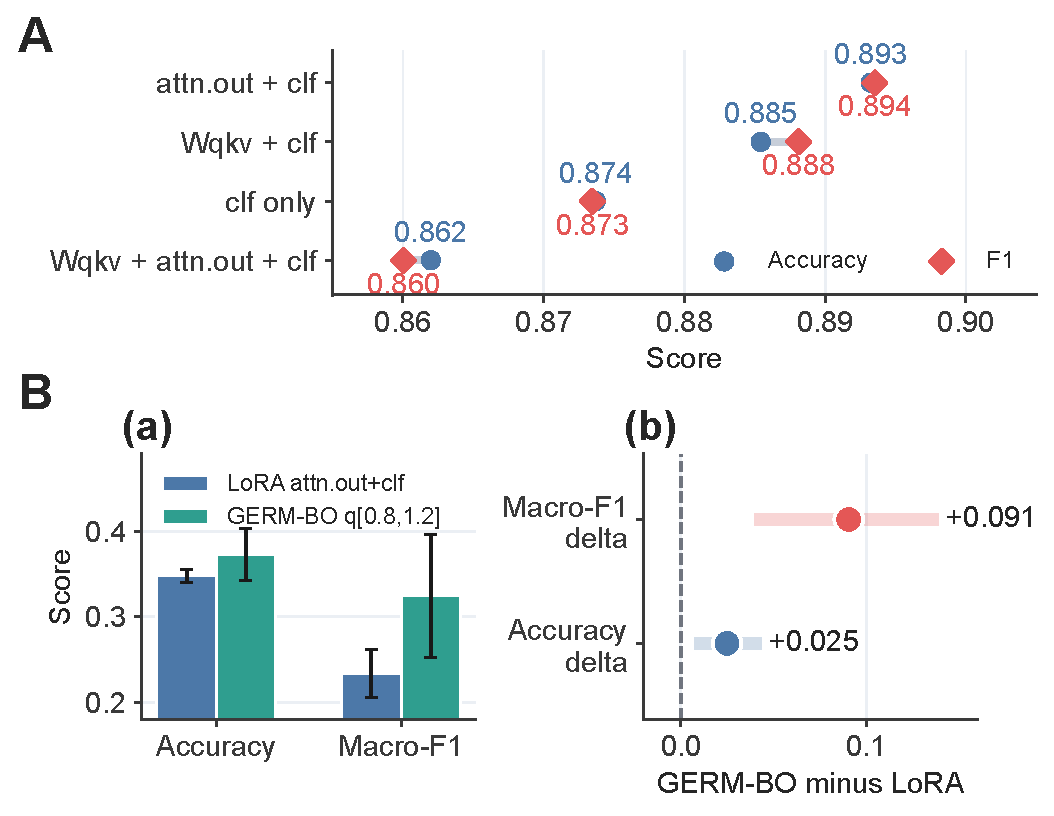
\includegraphics[width=0.85\linewidth]{0408.pdf}
\caption{Target-module ablation and external splice confirmation. \textbf{A}, target-module ablation in the controlled setting, visualized as a dumbbell comparison between accuracy and F1 for classifier-only, \modpath{Wqkv + classifier}, \modpath{attention.output + classifier}, and the fuller combined setting. The \modpath{attention.output + classifier} variant provides the strongest operating point. \textbf{B}, pooled confirmation on the strict \splitname{3-mer-balanced} splice split over seeds 50--59. The left panel reports pooled mean accuracy and macro-F1 for LoRA \modpath{attention.output + classifier} and GERM-BO with quantile-normalized compensation, while the right panel reports paired improvements with bootstrap confidence intervals. The macro-F1 gain is the more stable and discriminative signal.}
\label{fig:architecture_external_confirmation}
\end{figure}



\subsection*{Label-free scoring and strict splice benchmark}

\subsubsection*{Strict splice benchmark protocol}

Our initial experiments on \splitname{splice\_sites\_all} revealed two issues, as summarized in Fig.~\ref{fig:external_benchmark_overview} and Fig.~\ref{fig:splice_shortcut_and_comparison}. First, the original sequence-estimated score could saturate: a raw clipped estimator based on center-window JSD had clip-max rate $\approx 99.9\%$ and test score standard deviation $\approx 0.0026$, making compensation close to a constant rescaling. Second, the original larger splice split was strongly helped by short-range $3$-mer shortcuts. On that split, $3$-mer Logistic Regression reached macro-F1 $0.4293 \pm 0.0008$ and $3$-mer Linear SVM reached $0.4259 \pm 0.0019$, both stronger than the DNABERT-2-family models.

\begin{figure}[htbp]
\centering
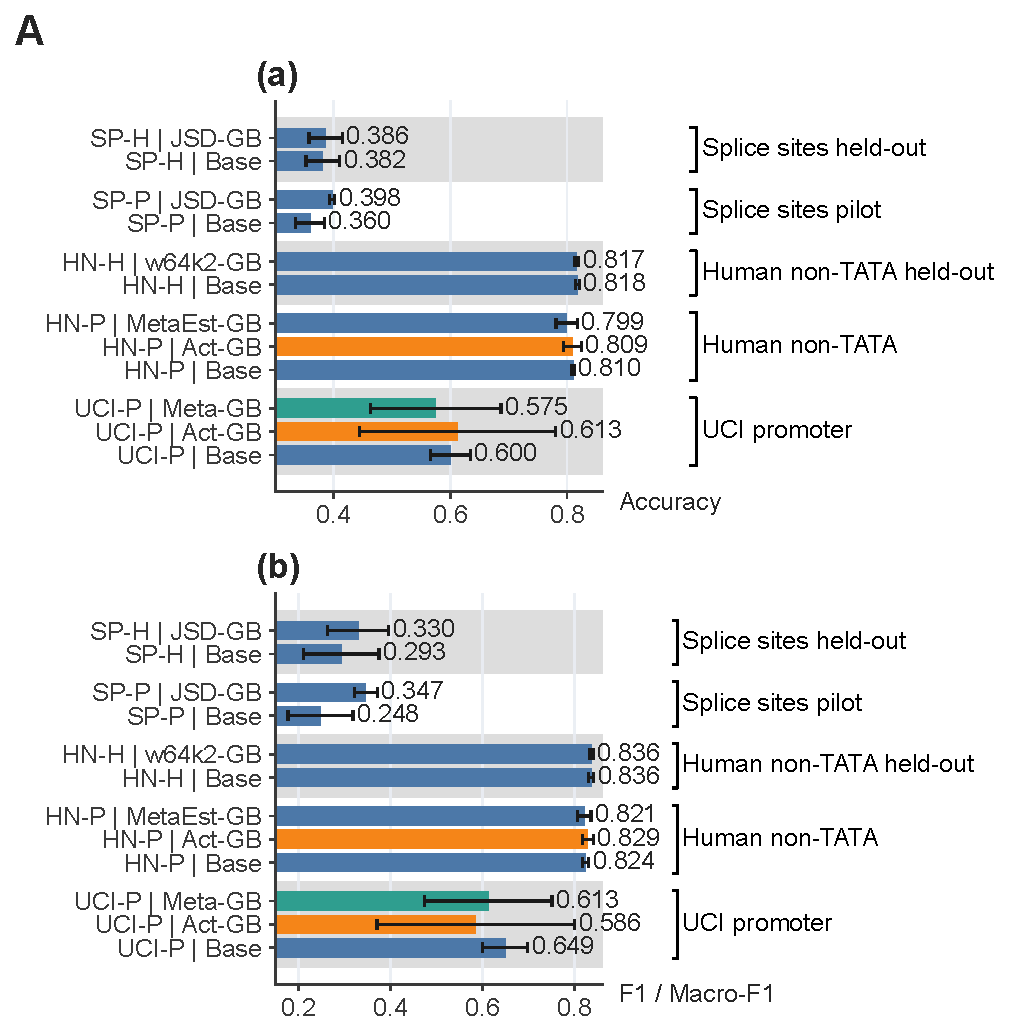
\includegraphics[width=0.85\linewidth]{05_external_benchmark_overview.pdf}
\caption{Overview of external pilot and held-out benchmarks. Results are shown for UCI promoter, \splitname{human\_nontata\_promoters}, and \splitname{splice\_sites\_all} datasets, with grouped horizontal comparisons for both accuracy and F1 / macro-F1. The comparison includes baseline LoRA, activation-derived GERM-BO, and metadata-driven GERM-BO variants.}
\label{fig:external_benchmark_overview}
\end{figure}



GC matching alone did not remove this effect. This behavior is illustrated in Fig.~\ref{fig:splice_shortcut_and_comparison}A, where shortcut-based models remain strong under the GC-matched split (GC-match) but degrade under the stricter 3-mer-balanced split (3-mer-bal). By contrast, on the stricter 3-mer-balanced split, the same baselines dropped to $0.4052 \pm 0.0023$ and $0.4128 \pm 0.0026$ macro-F1, respectively. We therefore adopt two changes in the final external protocol: (i) train-quantile normalization for the estimated border score, and (ii) evaluation on the strict \splitname{3-mer-balanced} split. The resulting evaluation protocol and its impact on model comparison are summarized in Fig.~\ref{fig:splice_shortcut_and_comparison}B.

\begin{figure}[htbp]
\centering
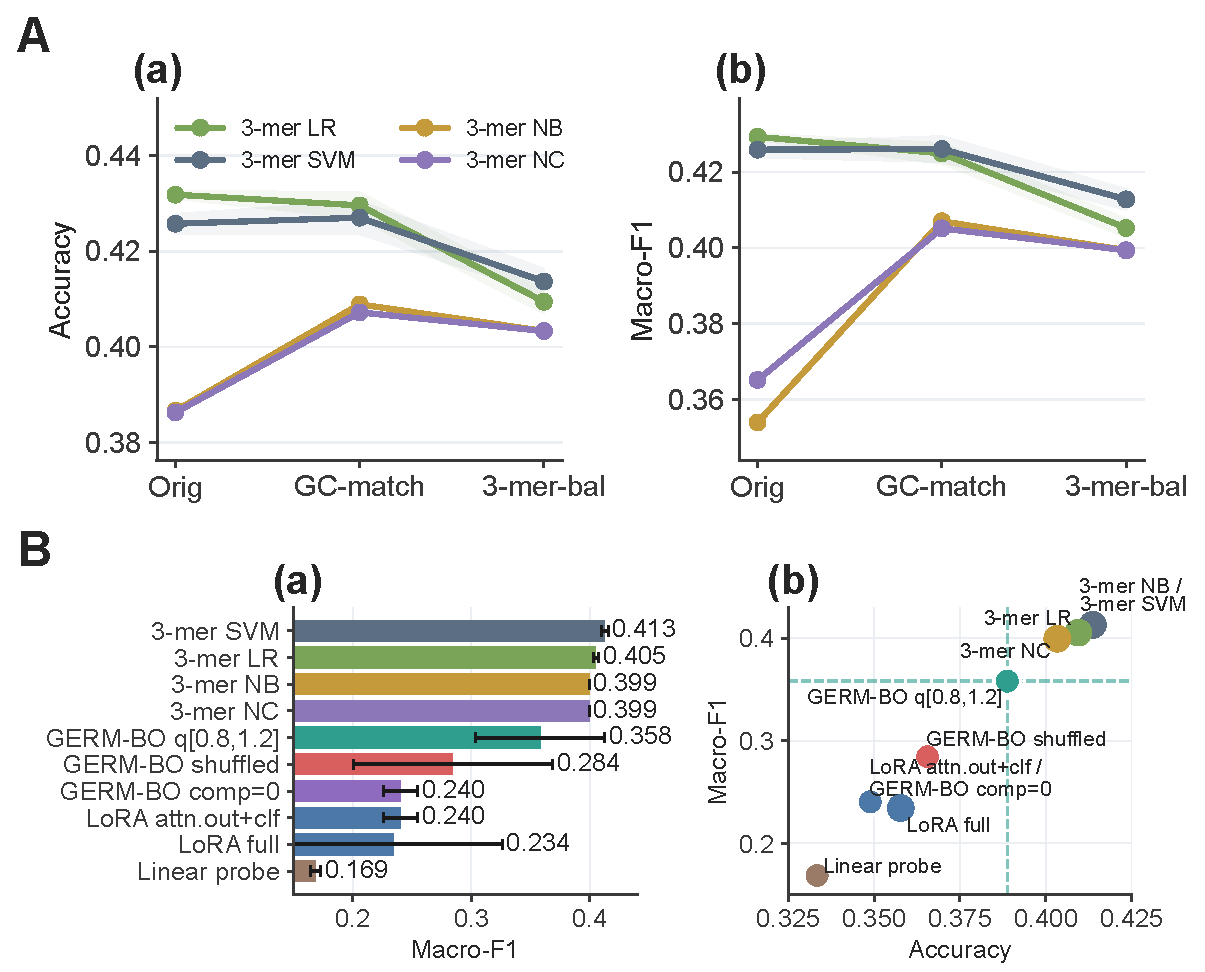
\includegraphics[width=0.85\linewidth]{0607.pdf}
\caption{Shortcut analysis and strict comparison on the splice benchmark. \textbf{A}, shortcut analysis showing performance of traditional 3-mer models across three data splits: original (Orig), GC-matched (GC-match), and 3-mer-balanced (3-mer-bal). GC matching alone does not substantially weaken the strongest 3-mer models, whereas the strict 3-mer-balanced split reduces shortcut strength more clearly. \textbf{B}, full comparison on the strict 3-mer-balanced split. The left panel ranks methods by macro-F1, while the right panel shows the accuracy--macro-F1 trade-off. Traditional 3-mer models remain strong in absolute score, but within the DNABERT-2 family, quantile-normalized GERM-BO provides the strongest result.}
\label{fig:splice_shortcut_and_comparison}
\end{figure}

Concretely, the final label-free score uses a center-window $k$-mer Jensen--Shannon divergence estimator (window 48, $k=2$, top-ratio 0.25) computed without labels, followed by train-quantile normalization to $[0.8,1.2]$ before clipping. The estimator uses the benchmark's shared center-position prior for all samples and never reads class labels when computing the score. Markov-background continuation estimates, repeat-aware failure modes, and tokenizer alignment details are provided in Document S1 and in the STAR Methods border-score subsection below.



\subsubsection*{External splice benchmark results}

Table~\ref{tab:external-main} reports the main external result on the strict \splitname{3-mer-balanced} splice split, pooled over seeds 50--59. The pooled comparison and paired improvements are further illustrated in Fig.~\ref{fig:architecture_external_confirmation}B. In the following, we use \textbf{LoRA-ATT} to denote the strongest LoRA baseline (applied to the \modpath{attention.output} and \modpath{classifier} modules), and \textbf{GERM-BO (Q)} to denote our method with quantile-normalized compensation (range $[0.8, 1.2]$, $\lambda_{\mathrm{comp}}=0.27$). We compare the strongest LoRA baseline and the final quantile-normalized GERM-BO configuration.

\begin{table}[htbp]
\centering
\caption{External main result on the strict \splitname{3-mer-balanced} splice split. Results are pooled over 10 random seeds (50--59). Method abbreviations are defined in the main text.}
\label{tab:external-main}
\small
\begin{tabular}{@{}lcc@{}}
\toprule
Method & Accuracy & Macro-F1 \\
\midrule
LoRA-ATT & $0.3476 \pm 0.0081$ & $0.2339 \pm 0.0282$ \\
GERM-BO (Q) & $\mathbf{0.3724 \pm 0.0302}$ & $\mathbf{0.3245 \pm 0.0715}$ \\
\bottomrule
\end{tabular}
\end{table}



The paired deltas are positive for both metrics, but the macro-F1 signal is more stable. Accuracy improves by $+0.0249$ with bootstrap $95\%$ confidence interval $[+0.0072, +0.0434]$, while macro-F1 improves by $+0.0906$ with bootstrap $95\%$ confidence interval $[+0.0396, +0.1392]$. The paired $t$-test $p$-values are $0.0115$ for accuracy and $0.0008$ for macro-F1. We therefore regard macro-F1 as the stronger external signal.

This result supports a narrower but important claim: on a stricter and more boundary-sensitive splice split, GERM-BO improves over strong DNABERT-2-family baselines. At the same time, we do not claim to beat all traditional sequence-only baselines. On the same strict split, $3$-mer Linear SVM still reaches $0.4137 \pm 0.0026$ accuracy and $0.4128 \pm 0.0026$ macro-F1.

\subsubsection*{Compensation ablation on the strict splice split}

To isolate the source of the external gain, Table~\ref{tab:external-ablation} compares the main DNABERT-2-family baselines on the strict splice split. The key observation is that \modpath{LoRA attention.output + classifier} and \modpath{GERM-BO comp=0} are numerically identical, whereas the compensated quantile-normalized variant is substantially stronger. This indicates that the gain is due to compensation rather than target-module choice alone.



Within the DNABERT-2 family, the result is internally consistent: compensation matters, shuffled metadata hurts, and the quantile-normalized metadata variant is the strongest model on macro-F1. The remaining gap to the best traditional $3$-mer baselines should therefore be interpreted as an external-benchmark limitation rather than as evidence against the mechanism itself.

\subsubsection*{Direction-aware PEFT baselines on the strict splice split}

To address whether the external gain is specific to metadata-aligned compensation, we compare GERM-BO (Q) against additional direction-reweighting baselines on the same strict split and seed protocol (50--54): a frozen DNABERT-2 linear probe, input-gated LoRA on \modpath{attention.output + classifier}, and activation-derived GERM-BO with $\lambda_{\mathrm{comp}}=0.27$. Table~\ref{tab:external-ablation} reports these comparisons together with the main LoRA and quantile-normalized GERM-BO results. Gated LoRA provides a matched-capacity baseline that reweights adapter updates from hidden states rather than from sequence-estimated border metadata. Activation-derived GERM-BO tests whether post-hoc activation scaling alone can reproduce the metadata-driven gain.

On seeds 50--54, GERM-BO (Q) reaches $0.3888 \pm 0.0233$ test accuracy and $0.3580 \pm 0.0545$ macro-F1, remaining the strongest DNABERT-2-family variant on macro-F1. Activation-derived GERM-BO reaches $0.3709 \pm 0.0144$ accuracy and $0.3112 \pm 0.0492$ macro-F1, improving over LoRA-ATT ($0.3489 \pm 0.0081$ accuracy; $0.2405 \pm 0.0145$ macro-F1) and gated LoRA ($0.3606 \pm 0.0254$; $0.2769 \pm 0.0873$) but falling short of the metadata-aligned quantile variant (paired macro-F1 gap $-0.0469$; bootstrap $95\%$ confidence interval $[-0.1170, +0.0311]$). Input-gated LoRA recovers a modest macro-F1 gain over uniform LoRA-ATT ($+0.0364$) yet remains below both compensated GERM-BO variants. These results separate border-aware compensation from generic hidden-state gating: direction reweighting alone is not sufficient to match metadata-aligned GERM-BO on the strict splice split.

\begin{table}[htbp]
\centering
\caption{External full comparison on the strict \splitname{3-mer-balanced} splice split.}
\label{tab:external-ablation}
\small
\begin{tabular}{lccc}
\toprule
Method & Family & Accuracy & Macro-F1 \\
\midrule
3-mer Linear SVM & Traditional & $\mathbf{0.4137 \pm 0.0026}$ & $\mathbf{0.4128 \pm 0.0026}$ \\
3-mer Logistic Regression & Traditional & $0.4094 \pm 0.0023$ & $0.4052 \pm 0.0023$ \\
3-mer Multinomial NB & Traditional & $0.4033 \pm 0.0000$ & $0.3994 \pm 0.0000$ \\
3-mer Nearest Centroid & Traditional & $0.4033 \pm 0.0000$ & $0.3994 \pm 0.0000$ \\
\midrule
GERM-BO quantile $[0.8,1.2]$ comp0.27 & DNABERT-2 + GERM-BO & $\mathbf{0.3888 \pm 0.0233}$ & $\mathbf{0.3580 \pm 0.0545}$ \\
GERM-BO activation-derived comp0.27 & DNABERT-2 + GERM-BO & $0.3709 \pm 0.0144$ & $0.3112 \pm 0.0492$ \\
GERM-BO shuffled metadata & DNABERT-2 + GERM-BO & $0.3656 \pm 0.0273$ & $0.2844 \pm 0.0842$ \\
Gated LoRA attention.output + classifier & DNABERT-2 + gated LoRA & $0.3606 \pm 0.0254$ & $0.2769 \pm 0.0873$ \\
LoRA attention.output + classifier & DNABERT-2 + LoRA & $0.3489 \pm 0.0081$ & $0.2405 \pm 0.0145$ \\
GERM-BO comp=0 & DNABERT-2 + GERM-BO & $0.3489 \pm 0.0081$ & $0.2405 \pm 0.0145$ \\
Baseline LoRA full target set & DNABERT-2 + LoRA & $0.3578 \pm 0.0334$ & $0.2344 \pm 0.0918$ \\
DNABERT-2 frozen linear probe & DNABERT-2 probe & $0.3334 \pm 0.0006$ & $0.1688 \pm 0.0042$ \\
\bottomrule
\end{tabular}
\end{table}

\subsubsection*{Class recovery on the strict splice split}

The external gain is not uniform across classes, as illustrated in Fig.~\ref{fig:why_it_works}A. Table~\ref{tab:class-recovery} summarizes the pooled per-class analysis over seeds 50--59. The main benefit comes from recovering non-dominant classes rather than further improving the dominant class.



The LoRA baseline collapses strongly toward class 2, whereas GERM-BO produces a much more balanced prediction distribution. This collapse and its correction by GERM-BO are clearly visualized in Fig.~\ref{fig:why_it_works}A. This class-recovery pattern is important for interpreting the external result: the gain comes primarily from restoring minority or boundary-sensitive classes rather than from trivially increasing confidence on the dominant class. Additional analysis of estimator quality and its relationship to sequence features is provided in Fig.~\ref{fig:why_it_works}B.

\begin{figure}[htbp]
\centering
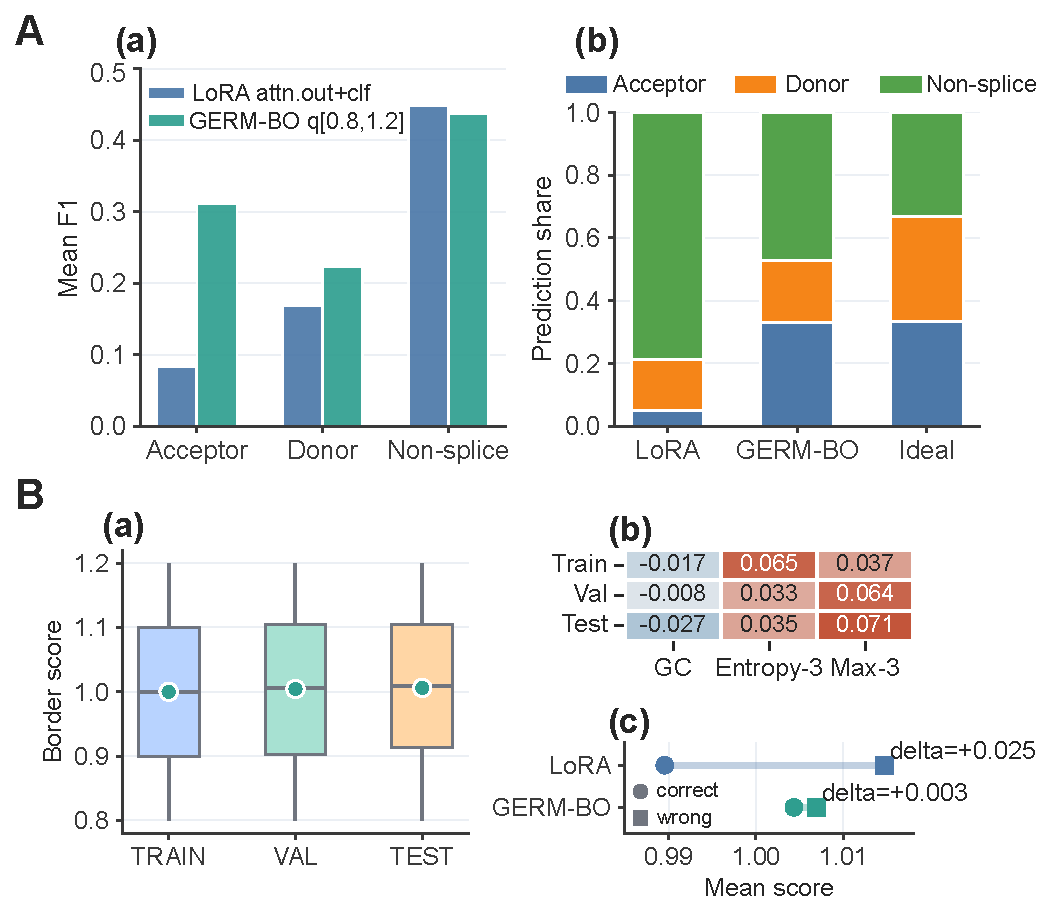
\includegraphics[width=0.85\linewidth]{0910.pdf}
\caption{Class recovery and estimator quality on the strict splice split. \textbf{A}, class-wise behavior on pooled seeds 50--59. The left panel compares per-class F1, showing that GERM-BO improves the non-dominant classes more strongly than the dominant class. The right panel shows prediction composition, demonstrating that the LoRA baseline collapses toward the dominant class while GERM-BO produces a more balanced prediction distribution. \textbf{B}, estimator-quality analysis for the strict split. Panel \textbf{B(a)} summarizes the train/validation/test score distributions with box-style quantile ranges and mean markers. Panel \textbf{B(b)} reports correlations between the estimator and simple sequence-composition proxies, indicating that the quantile-normalized estimator is not merely a trivial GC or $3$-mer shortcut. Panel \textbf{B(c)} compares score means for correct and wrong predictions, showing that the estimator is not a strong standalone error detector and is better interpreted as a compensation signal.}
\label{fig:why_it_works}
\end{figure}

\begin{table}[htbp]
\centering
\caption{Per-class performance and prediction distribution on the strict splice split (seeds 50--59).}
\label{tab:class-recovery}
\small
\setlength{\tabcolsep}{6pt}
\begin{tabular}{lcccccc}
\toprule
& \multicolumn{3}{c}{F1 score} & \multicolumn{3}{c}{Prediction count} \\
\cmidrule(lr){2-4} \cmidrule(lr){5-7}
Class & LoRA & GERM-BO & $\Delta$ & LoRA & GERM-BO & $\Delta$ \\
\midrule
Acceptor    & 0.0842 & \textbf{0.3121} & +0.2280 & 91.5   & 593.2  & +501.7 \\
Donor       & 0.1684 & \textbf{0.2233} & +0.0549 & 293.1  & 354.9  & +61.8  \\
Non-splice  & \textbf{0.4492} & 0.4380 & -0.0112 & 1415.4 & 851.9  & -563.5 \\
\bottomrule
\end{tabular}
\end{table}

\subsection*{Scope across additional genomic tasks}

\subsubsection*{Secondary promoter benchmark}

Beyond splice sites, we evaluate label-free border-score estimation on the Genomic Benchmarks \splitname{human\_nontata\_promoters} task (held-out seeds 45--49; pilot subset 2000/500/1000). Baseline LoRA reaches $0.8178 \pm 0.0034$ test accuracy, whereas metadata-estimated GERM-BO with the best label-free estimator ($w=64$, $k=2$, top-ratio 0.10) reaches $0.8168 \pm 0.0032$ accuracy. The paired difference is negligible ($\Delta=-0.0010$ accuracy), indicating that the current sequence-estimated score is not yet strong enough to improve over LoRA on this promoter task despite the controlled mechanism result. This null external outcome motivates the stricter splice protocol above and is summarized alongside UCI promoter pilots in Fig.~\ref{fig:external_benchmark_overview}.

\subsubsection*{Nucleotide Transformer chromatin and regulatory pilots}

To extend beyond promoters and splice sites, we evaluate all ten histone ChIP-seq peak tasks plus \splitname{enhancers} from the Nucleotide Transformer downstream collection~\cite{nucleotidetransformer2024} (500\,bp histone windows; $\approx$200\,bp enhancer windows; pilot subset 2000/500/1000). The public release does not include standalone TFBS labels, so \splitname{enhancers} serves as the closest regulatory benchmark in this repository. All pilots use real DNABERT-2, train-quantile center-window k-mer JSD metadata, and argmax test evaluation. Table~\ref{tab:histone-dnabert-pilots} reports pilot (seeds 42--44) and held-out (seeds 45--49) accuracy means and paired GERM-BO minus LoRA deltas.

On pilot seeds 42--44, metadata-estimated GERM-BO shows a positive mean accuracy delta on seven of ten histone marks. The clearest gain is on \splitname{H3K14ac} (LoRA $0.5923 \pm 0.0816$ vs.\ GERM-BO $0.6650 \pm 0.0156$ accuracy; paired $\Delta=+0.0727$; bootstrap $95\%$ confidence interval $[+0.0000, +0.1570]$). Smaller positive deltas appear on \splitname{H3K4me2} ($\Delta=+0.0310$), \splitname{H3K9ac} ($+0.0310$), and \splitname{H3K36me3} ($+0.0167$), whereas \splitname{H4} ($\Delta=-0.0513$; CI excludes zero) and \splitname{H3K4me1} ($-0.0147$) favor LoRA.

Held-out confirmation on seeds 45--49 does not replicate the pilot pattern. Across histone marks, six of ten tasks show a positive mean delta, but no task has a bootstrap confidence interval excluding zero. \splitname{H3K14ac} reverses to near-null ($\Delta=-0.0060$; CI $[-0.0346, +0.0206]$), and \splitname{H4} flips sign ($\Delta=+0.0544$). Only four of eleven tasks show the same sign in pilot and held-out splits.

\begin{table}[p]
\centering
\caption{DNABERT-2 chromatin and regulatory pilots with label-free border metadata (pilot seeds 42--44 vs.\ held-out seeds 45--49).}
\label{tab:histone-dnabert-pilots}
\footnotesize
\setlength{\tabcolsep}{3pt}
\begin{tabular}{llcccccc}
\toprule
Task & Cat. & LoRA (pilot) & GERM-BO (pilot) & $\Delta$ pilot [95\% CI] & LoRA (held-out) & GERM-BO (held-out) & $\Delta$ held-out [95\% CI] \\
\midrule
H3 & histone & 0.7750 & 0.7833 & $+0.0083$ [$-0.1390$, $+0.1310$] & 0.8182 & 0.7640 & $-0.0542$ [$-0.1922$, $+0.0316$] \\
H3K14ac & histone & 0.5923 & 0.6650 & $+0.0727$ [$+0.0000$, $+0.1570$] & 0.6654 & 0.6594 & $-0.0060$ [$-0.0346$, $+0.0206$] \\
H3K36me3 & histone & 0.6843 & 0.7010 & $+0.0167$ [$-0.0410$, $+0.1000$] & 0.7038 & 0.7084 & $+0.0046$ [$-0.0228$, $+0.0404$] \\
H3K4me1 & histone & 0.6733 & 0.6587 & $-0.0147$ [$-0.0260$, $-0.0080$] & 0.6380 & 0.6522 & $+0.0142$ [$-0.0028$, $+0.0310$] \\
H3K4me2 & histone & 0.5927 & 0.6237 & $+0.0310$ [$-0.0350$, $+0.1220$] & 0.6262 & 0.6328 & $+0.0066$ [$-0.0148$, $+0.0300$] \\
H3K4me3 & histone & 0.5410 & 0.5527 & $+0.0117$ [$-0.0880$, $+0.0620$] & 0.5568 & 0.5536 & $-0.0032$ [$-0.0370$, $+0.0302$] \\
H3K79me3 & histone & 0.7430 & 0.7560 & $+0.0130$ [$-0.0150$, $+0.0580$] & 0.7356 & 0.7342 & $-0.0014$ [$-0.0558$, $+0.0648$] \\
H3K9ac & histone & 0.6590 & 0.6900 & $+0.0310$ [$-0.0170$, $+0.1220$] & 0.6544 & 0.6794 & $+0.0250$ [$-0.0194$, $+0.0666$] \\
H4 & histone & 0.8793 & 0.8280 & $-0.0513$ [$-0.1110$, $-0.0110$] & 0.7998 & 0.8542 & $+0.0544$ [$-0.0162$, $+0.1338$] \\
H4ac & histone & 0.6383 & 0.6310 & $-0.0073$ [$-0.0330$, $+0.0120$] & 0.5768 & 0.5774 & $+0.0006$ [$-0.0462$, $+0.0404$] \\
enhancers & regulatory & 0.7217 & 0.7292 & $+0.0075$ [$-0.0125$, $+0.0450$] & 0.7395 & 0.7325 & $-0.0070$ [$-0.0150$, $+0.0010$] \\
\bottomrule
\end{tabular}

Pilot subset 2000/500/1000 from \texttt{InstaDeepAI/nucleotide\_transformer\_downstream\_tasks}. Test accuracy means over three or five seeds. No held-out task has a bootstrap confidence interval excluding zero.
\end{table}

We further replicate the same histone pilot protocol on the Nucleotide Transformer v2 50M backbone (seeds 42--44; Table~\ref{tab:histone-nt-pilot}). Metadata-estimated GERM-BO shows a positive mean delta on only three of ten histone marks, with the largest gain on \splitname{H4ac} ($\Delta=+0.0130$; CI $[+0.0080, +0.0180]$) and near-null behavior on \splitname{H3K14ac} ($\Delta=-0.0023$). Sign agreement with DNABERT-2 is limited (four of ten tasks). Taken together, chromatin and regulatory pilots do not establish a robust metadata-estimation advantage outside the boundary-sensitive splice setting.

\begin{table}[p]
\centering
\caption{Nucleotide Transformer v2 50M histone-mark pilot with label-free border metadata (seeds 42--44).}
\label{tab:histone-nt-pilot}
\footnotesize
\setlength{\tabcolsep}{4pt}
\begin{tabular}{lcccc}
\toprule
Task & NT LoRA Acc & NT GERM-BO Acc & $\Delta$ Acc [95\% CI] & DNABERT-2 $\Delta$ Acc (pilot) \\
\midrule
H3 & 0.7917 & 0.7880 & $-0.0037$ [$-0.0070$, $+0.0000$] & $+0.0083$ \\
H3K14ac & 0.6307 & 0.6283 & $-0.0023$ [$-0.0100$, $+0.0030$] & $+0.0727$ \\
H3K36me3 & 0.6813 & 0.6767 & $-0.0047$ [$-0.0110$, $+0.0010$] & $+0.0167$ \\
H3K4me1 & 0.6167 & 0.6153 & $-0.0013$ [$-0.0050$, $+0.0020$] & $-0.0147$ \\
H3K4me2 & 0.6020 & 0.6060 & $+0.0040$ [$+0.0000$, $+0.0110$] & $+0.0310$ \\
H3K4me3 & 0.5657 & 0.5643 & $-0.0013$ [$-0.0070$, $+0.0020$] & $+0.0117$ \\
H3K79me3 & 0.7333 & 0.7340 & $+0.0007$ [$-0.0020$, $+0.0030$] & $+0.0130$ \\
H3K9ac & 0.6530 & 0.6483 & $-0.0047$ [$-0.0080$, $+0.0000$] & $+0.0310$ \\
H4 & 0.8423 & 0.8373 & $-0.0050$ [$-0.0120$, $+0.0000$] & $-0.0513$ \\
H4ac & 0.5837 & 0.5967 & $+0.0130$ [$+0.0080$, $+0.0180$] & $-0.0073$ \\
\bottomrule
\end{tabular}

Same pilot protocol as Table~\ref{tab:histone-dnabert-pilots}. NT v2 50M shows a positive mean GERM-BO delta on three of ten histone marks; sign agreement with DNABERT-2 is four of ten tasks.
\end{table}

\subsection*{Sensitivity, resource footprint, and backbone transfer}



\subsubsection*{Hyperparameter sensitivity and resource footprint}

We report additional analyses requested for reproducibility and scope: sensitivity to $\lambda_{\mathrm{comp}}$ and rank $r$, and a quantitative resource snapshot relative to LoRA (Table~\ref{tab:comp-sensitivity}).

\subsubsection*{Compensation strength $\lambda_{\mathrm{comp}}$.}
Panel~(a) in Table~\ref{tab:comp-sensitivity} summarizes a grid over $\lambda_{\mathrm{comp}} \in \{0.15,0.20,0.25,0.27\}$ on held-out \splitname{border\_medium} and \splitname{border\_hard} with metadata-driven compensation (five seeds each). Performance is stable across a moderate range; $\lambda_{\mathrm{comp}}=0.27$ is near-optimal on \splitname{border\_hard} and competitive on \splitname{border\_medium}, supporting our main-setting choice without sharp sensitivity.

\subsubsection*{Rank budget $r$.}
Panel~(b) reports metadata-driven GERM-BO on \splitname{border\_hard} for $r \in \{4,8,16\}$ with fixed $\lambda_{\mathrm{comp}}=0.27$ (three seeds). Accuracy is stable across moderate ranks, indicating that the gain is not driven by a narrow rank sweet spot; $r=8$ remains the default for parity with LoRA baselines.

\subsubsection*{Resource footprint.}
Panel~(c) profiles the strict \splitname{3-mer-balanced} splice setting (seed 50, batch size 4, seq length 512). GERM-BO uses the same trainable parameter count as LoRA because compensation is a multiplicative gate on the LoRA branch rather than additional adapter weights. Peak GPU memory from forward snapshots differs by less than $1\%$; end-to-end training time per run is comparable (LoRA: 223\,s on seed 50) because compensation adds only elementwise scaling on the LoRA branch.

\begin{table}[htbp]
\centering
\caption{Hyperparameter sensitivity and resource footprint.}
\label{tab:comp-sensitivity}\label{tab:rank-sensitivity}\label{tab:resource-footprint}
\footnotesize
\setlength{\tabcolsep}{3pt}
\begin{minipage}[t]{0.50\textwidth}
\centering
\textbf{(a)} Compensation strength\\[2pt]
\begin{tabular}{@{}lcc@{}}
\toprule
$\lambda_{\mathrm{comp}}$ & \splitname{border\_medium} & \splitname{border\_hard} \\
\midrule
0.15 & $0.9070 \pm 0.0218$ & $0.8469 \pm 0.0173$ \\
0.20 & $0.8992 \pm 0.0476$ & $0.8609 \pm 0.0278$ \\
0.25 & $0.8484 \pm 0.0829$ & $0.8516 \pm 0.0390$ \\
0.27 & $0.8930 \pm 0.0557$ & $\mathbf{0.8695 \pm 0.0202}$ \\
\bottomrule
\end{tabular}
\vspace{6pt}

\textbf{(b)} LoRA rank $r$\\[2pt]
\begin{tabular}{@{}lc@{}}
\toprule
$r$ & Test accuracy \\
\midrule
4  & $0.9115 \pm 0.0784$ \\
8  & $0.9193 \pm 0.0695$ \\
16 & $0.9922 \pm 0.0084$ \\
\bottomrule
\end{tabular}
\end{minipage}\hfill
\begin{minipage}[t]{0.44\textwidth}
\centering
\textbf{(c)} Resource footprint\\[2pt]
\begin{tabular}{@{}lccc@{}}
\toprule
Method & Params & Mem (MB) & Time (s) \\
\midrule
LoRA-ATT & 30{,}744 & 587 & 223 \\
GERM-BO (Q) & 30{,}744 & 587 & 171 \\
\bottomrule
\end{tabular}
\end{minipage}

Panel \textbf{(a)}, compensation strength $\lambda_{\mathrm{comp}}$ on held-out controlled splits (five seeds; test accuracy mean $\pm$ std). Panel \textbf{(b)}, LoRA rank $r$ on \splitname{border\_hard} (metadata compensation, three seeds). Panel \textbf{(c)}, resource footprint on the strict splice split (seed 50).
\end{table}

\subsubsection*{Cross-backbone replication on \splitname{border\_hard}}

To test whether the compensation mechanism is backbone-specific, we replicate the oracle-metadata \splitname{border\_hard} protocol on Nucleotide Transformer v2 50M~\cite{nucleotidetransformer2024} and HyenaDNA tiny~\cite{hyenadna2024} (held-out seeds 50--54; rank 8; $\lambda_{\mathrm{comp}}=0.27$; Table~\ref{tab:cross-backbone-oracle}). On NT v2 50M, LoRA reaches $0.8945 \pm 0.0124$ test accuracy and macro-F1, whereas metadata-driven GERM-BO reaches $0.9828 \pm 0.0045$ (paired $\Delta=+0.0883$). On HyenaDNA tiny, LoRA reaches $0.9625 \pm 0.0090$, whereas GERM-BO reaches $0.9945 \pm 0.0021$ (paired $\Delta=+0.0320$). These gains confirm that border-aware compensation transfers beyond DNABERT-2 under oracle border scores on the controlled hard split.

\begin{table}[htbp]
\centering
\caption{Cross-backbone replication on oracle-metadata \splitname{border\_hard} (seeds 50--54).}
\label{tab:cross-backbone-oracle}
\small
\begin{tabular}{lccc}
\toprule
Backbone / Method & Seeds & Accuracy & Macro-F1 \\
\midrule
NT v2 50M LoRA & 5 & $0.8945 \pm 0.0124$ & $0.8944 \pm 0.0124$ \\
NT v2 50M GERM-BO (Meta) & 5 & $\mathbf{0.9828 \pm 0.0045}$ & $\mathbf{0.9828 \pm 0.0045}$ \\
HyenaDNA tiny LoRA & 5 & $0.9625 \pm 0.0090$ & $0.9625 \pm 0.0090$ \\
HyenaDNA tiny GERM-BO (Meta) & 5 & $\mathbf{0.9945 \pm 0.0021}$ & $\mathbf{0.9945 \pm 0.0021}$ \\
\bottomrule
\end{tabular}

Paired GERM-BO minus LoRA: NT v2 50M $\Delta=+0.0883$ accuracy; HyenaDNA tiny $\Delta=+0.0320$ accuracy. Rank 8, $\lambda_{\mathrm{comp}}=0.27$, oracle metadata border scores.
\end{table}

We next ask whether the same transfer holds on the strict \splitname{3-mer-balanced} splice split with label-free train-quantile border metadata (seeds 50--54; Table~\ref{tab:cross-backbone-splice-label-free}). DNABERT-2 GERM-BO improves over LoRA by $+0.0399$ accuracy and $+0.1176$ macro-F1 (bootstrap $95\%$ confidence intervals exclude zero). NT v2 50M shows a smaller mean gain ($+0.0290$ accuracy; $+0.0307$ macro-F1) with bootstrap confidence intervals crossing zero, despite a higher absolute LoRA baseline ($0.6447 \pm 0.0865$ accuracy). HyenaDNA tiny is near-null ($\Delta=-0.0024$ accuracy and macro-F1). Thus backbone generality is setting-dependent: compensation transfers strongly under oracle scores and on DNABERT-2 with label-free splice estimation, but is not yet robust on alternative backbones under the same label-free protocol.

\begin{table}[p]
\centering
\caption{Cross-backbone replication on the strict \splitname{3-mer-balanced} splice split with label-free border metadata (seeds 50--54).}
\label{tab:cross-backbone-splice-label-free}
\small
\setlength{\tabcolsep}{4pt}
\begin{tabular}{lcccccc}
\toprule
Backbone & LoRA Acc & GERM-BO Acc & LoRA Macro-F1 & GERM-BO Macro-F1 & $\Delta$ Acc [95\% CI] & $\Delta$ F1 [95\% CI] \\
\midrule
DNABERT-2 & $0.3489 \pm 0.0081$ & $\mathbf{0.3888 \pm 0.0233}$ & $0.2405 \pm 0.0145$ & $\mathbf{0.3580 \pm 0.0545}$ & $+0.0399$ [$+0.0257$, $+0.0541$] & $+0.1176$ [$+0.0620$, $+0.1618$] \\
NT v2 50M & $0.6447 \pm 0.0865$ & $0.6737 \pm 0.0837$ & $0.6393 \pm 0.0859$ & $0.6700 \pm 0.0857$ & $+0.0290$ [$-0.0038$, $+0.0862$] & $+0.0307$ [$-0.0065$, $+0.0948$] \\
HyenaDNA tiny & $0.6088 \pm 0.0249$ & $0.6063 \pm 0.0214$ & $0.6031 \pm 0.0277$ & $0.6007 \pm 0.0248$ & $-0.0024$ [$-0.0078$, $+0.0028$] & $-0.0024$ [$-0.0085$, $+0.0036$] \\
\bottomrule
\end{tabular}

Train-quantile center-window k-mer JSD metadata, quantile clip $[0.8,1.2]$, $\lambda_{\mathrm{comp}}=0.27$. Bootstrap confidence intervals from paired seed deltas.
\end{table}



\section*{DISCUSSION}

\subsection*{Limitations of the study}

\noindent\emph{Theoretical scope.} Theorem~\ref{thm:fisher} uses simplifying scale and independence assumptions. Activation-level calibration on both random-init and fine-tuned checkpoints confirms the predicted border ordering of $R_w(\tau)$ on key controlled settings (notably trained GERM-BO on \splitname{border\_hard} and trained LoRA on \splitname{hard\_border\_large}), but the signal is model- and split-dependent; the trainer still uses Equation~\eqref{eq:implcomp} rather than a token-wise $\Gamma$ derived from calibrated $\tau$.

\emph{Backbone and task scope.} Main external benchmarks use DNABERT-2. Cross-backbone replication on oracle-metadata \splitname{border\_hard} confirms compensation on Nucleotide Transformer v2 50M and HyenaDNA tiny, but the same label-free strict-splice protocol yields robust GERM-BO gains only on DNABERT-2; NT v2 50M shows inconclusive mean deltas and HyenaDNA tiny is near-null. Label-free histone-mark pilots and held-out confirmation (seeds 45--49) likewise do not establish a robust metadata-estimation advantage outside the DNABERT-2 strict splice setting. External splice gains remain modest relative to strong $3$-mer baselines.

\emph{Remaining comparisons.} Mixture-of-adapters and task-vector reweighting~\cite{stickland2019bert,ilharco2022editing,he2022unified} remain future work. The public Nucleotide Transformer downstream release does not provide standalone TFBS labels; dedicated TF motif benchmarks remain outside the current scope.

\subsection*{Summary and outlook}

We presented GERM-BO, a reproducible border-aware adapter framework for resource-efficient genomic foundation models under outlier suppression. The key claim is that genomic word overlap is not a peripheral detail for adaptation. It generates clustered occurrences, inflates token-specific burst statistics, and can therefore make outlier suppression selectively remove adaptation information from high-border directions. We formalized this effect as border-burst suppression and used it to design a LoRA-compatible compensation channel. Controlled experiments establish the mechanism under oracle border scores, direction-aware PEFT baselines clarify that metadata-aligned compensation outperforms generic adapter gating on the strict splice split, and promoter, chromatin, and enhancer pilots delineate where label-free estimation remains insufficient.

Next steps are vocabulary-aligned token--word mapping for $\Gamma$, stronger label-free estimators on repeat-rich real genomes, and dedicated TFBS benchmarks beyond the public Nucleotide Transformer downstream release.


\newpage

\section*{RESOURCE AVAILABILITY}

\subsection*{Lead contact}
Requests for further information and resources should be directed to and will be fulfilled by the lead contact, Mingxuan Huang (1262569430@qq.com).

\subsection*{Materials availability}
This study did not generate new unique reagents.

\subsection*{Data and code availability}
\begin{itemize}
  \item Public raw sequence data used in this study are available from the UCI Molecular Biology Promoter Gene Sequences repository (\url{https://archive.ics.uci.edu/ml/machine-learning-databases/molecular-biology/promoter-gene-sequences/promoters.data}), Genomic Benchmarks \texttt{human\_nontata\_promoters} (version 0; \url{https://github.com/ML-Bioinfo-CEITEC/genomic_benchmarks}), Hugging Face Datasets \texttt{simecek/human\_nontata\_promoters} (\url{https://huggingface.co/datasets/simecek/human_nontata_promoters}), and the Nucleotide Transformer downstream task repository \texttt{InstaDeepAI/nucleotide\_transformer\_downstream\_tasks}~\cite{nucleotidetransformer2024} (\url{https://huggingface.co/datasets/InstaDeepAI/nucleotide_transformer_downstream_tasks}). The pretrained DNABERT-2 (117M) backbone is available as \texttt{zhihan1996/DNABERT-2-117M}~\cite{dnabert22023} (\url{https://huggingface.co/zhihan1996/DNABERT-2-117M}).
  \item Reviewer-accessible code and processed data will be provided at submission at \url{https://github.com/hhhhmx/GERM-BO.git}. This repository should include the GERM-BO adapter implementation, training and evaluation entry points, split-preparation scripts, YAML configurations for all reported runs, processed train/validation/test splits for the controlled border-aware tasks and the strict \splitname{3-mer-balanced} splice benchmark, and scripts for regenerating the reported tables and figures.
  \item A permanent public archive with DOI will be created before publication at \url{[ARCHIVE_DOI_URL_TO_BE_ADDED]}. Until the archive is active, all materials required to reproduce the reported analyses are available from the lead contact upon reasonable request.
\end{itemize}

\section*{ACKNOWLEDGMENTS}
We thank our research group and advisors for helpful discussions and feedback on this manuscript. We gratefully acknowledge the maintainers of the UCI Machine Learning Repository, Genomic Benchmarks, Hugging Face, and the Nucleotide Transformer downstream benchmark collection for publicly releasing the sequence datasets and model checkpoints used in this study. Computational experiments were performed using institutional GPU computing resources.

\section*{AUTHOR CONTRIBUTIONS}
Conceptualization, J.W. and Y.S.; methodology, M.H., J.W., and Y.S.; software, M.H.; investigation, M.H.; visualization, M.H.; writing--original draft, M.H. and Y.S.; writing--review \& editing, M.H., J.W., and Y.S.; supervision, J.W. and Y.S.

\section*{DECLARATION OF INTERESTS}
The authors declare no competing interests.

\section*{SUPPLEMENTAL INFORMATION INDEX}
\begin{description}
  \item Document S1. Mathematical proofs, theory-to-implementation mapping, and Markov-background estimator details (supplemental\_proofs.pdf)
  \item Key resources table. Reagents, datasets, and software (KRT6a38985775af2.docx)
\end{description}

\bibliography{references}

\newpage

\section*{STAR METHODS}

\subsection*{Key resources table}
The key resources table (KRT) for this study is provided as a separate file (\texttt{KRT6a38985775af2.docx}; submission ID: KRT6a38985775af2). Items listed in the KRT are also described in the method details below and in the \emph{Data and code availability} statement.

\subsection*{Experimental model and study participant details}
This is a computational study using publicly available DNA sequence benchmarks and a pretrained DNABERT-2 genomic language model. No human participants or experimental organisms were used.

\subsection*{Method details}

\subsubsection*{Backbone and adapters}
All experiments use DNABERT-2 (117M) with LoRA-style adapters on \modpath{attention.output + classifier} unless otherwise stated. GERM-BO applies sample-level multiplicative compensation on the LoRA branch (Equation~\eqref{eq:implcomp}) using metadata, activation-derived, or sequence-estimated border scores.

\subsubsection*{Controlled and external benchmarks}
Controlled tasks use synthetic border-aware splits (\splitname{border\_easy}, \splitname{border\_medium}, \splitname{border\_hard}, \splitname{hard\_border\_large}). External evaluation uses the strict \splitname{3-mer-balanced} splice split derived from \splitname{splice\_sites\_all}.

\subsubsection*{Border score channels and estimation}
Controlled experiments use metadata border scores generated with the task splits. External experiments use label-free sequence-estimated scores (center-window k-mer divergence with optional train-quantile normalization) or activation-derived scores as described in the Results. The Markov-background estimator $\widehat{\rho}_w$, tokenizer alignment details, and repeat-aware failure modes are specified in Document S1 and \texttt{METADATA\_SCORE\_DEFINITION.md} in the code release. Readers should consult those materials for estimator robustness and for run-level hyperparameters not repeated in the main tables.

\subsubsection*{Training protocol}
Training uses a single GPU, AdamW optimization, early stopping on validation accuracy, and multiple random seeds as reported in each table. Default LoRA rank $r=8$, scaling $\alpha=16$, and compensation strength $\lambda_{\mathrm{comp}}=0.27$ unless varied in sensitivity analyses. The reviewer repository will include exact commands for the mock-data smoke test, controlled validation, strict splice evaluation, and table-generation scripts.

\subsection*{Quantification and statistical analysis}
Binary controlled tasks report test accuracy and F1; the splice benchmark reports accuracy and macro-F1 as mean $\pm$ standard deviation across seeds. Key pairwise comparisons use paired bootstrap 95\% confidence intervals and paired $t$-tests where reported in the Results.

\subsection*{Additional resources}
Public raw data sources are listed under \emph{Data and code availability} above. The pretrained backbone (\texttt{zhihan1996/DNABERT-2-117M}), external benchmarks (UCI Promoter, Genomic Benchmarks \texttt{human\_nontata\_promoters}, and \texttt{splice\_sites\_all}), and all split-preparation scripts are documented in the reviewer repository described above.

\end{document}
